\documentclass{beamer}\usepackage[]{graphicx}\usepackage[]{color}
%% maxwidth is the original width if it is less than linewidth
%% otherwise use linewidth (to make sure the graphics do not exceed the margin)
\makeatletter
\def\maxwidth{ %
  \ifdim\Gin@nat@width>\linewidth
    \linewidth
  \else
    \Gin@nat@width
  \fi
}
\makeatother

\definecolor{fgcolor}{rgb}{0.196, 0.196, 0.196}
\newcommand{\hlnum}[1]{\textcolor[rgb]{0.063,0.58,0.627}{#1}}%
\newcommand{\hlstr}[1]{\textcolor[rgb]{0.063,0.58,0.627}{#1}}%
\newcommand{\hlcom}[1]{\textcolor[rgb]{0.588,0.588,0.588}{#1}}%
\newcommand{\hlopt}[1]{\textcolor[rgb]{0.196,0.196,0.196}{#1}}%
\newcommand{\hlstd}[1]{\textcolor[rgb]{0.196,0.196,0.196}{#1}}%
\newcommand{\hlkwa}[1]{\textcolor[rgb]{0.231,0.416,0.784}{#1}}%
\newcommand{\hlkwb}[1]{\textcolor[rgb]{0.627,0,0.314}{#1}}%
\newcommand{\hlkwc}[1]{\textcolor[rgb]{0,0.631,0.314}{#1}}%
\newcommand{\hlkwd}[1]{\textcolor[rgb]{0.78,0.227,0.412}{#1}}%
\let\hlipl\hlkwb

\usepackage{framed}
\makeatletter
\newenvironment{kframe}{%
 \def\at@end@of@kframe{}%
 \ifinner\ifhmode%
  \def\at@end@of@kframe{\end{minipage}}%
  \begin{minipage}{\columnwidth}%
 \fi\fi%
 \def\FrameCommand##1{\hskip\@totalleftmargin \hskip-\fboxsep
 \colorbox{shadecolor}{##1}\hskip-\fboxsep
     % There is no \\@totalrightmargin, so:
     \hskip-\linewidth \hskip-\@totalleftmargin \hskip\columnwidth}%
 \MakeFramed {\advance\hsize-\width
   \@totalleftmargin\z@ \linewidth\hsize
   \@setminipage}}%
 {\par\unskip\endMakeFramed%
 \at@end@of@kframe}
\makeatother

\definecolor{shadecolor}{rgb}{.97, .97, .97}
\definecolor{messagecolor}{rgb}{0, 0, 0}
\definecolor{warningcolor}{rgb}{1, 0, 1}
\definecolor{errorcolor}{rgb}{1, 0, 0}
\newenvironment{knitrout}{}{} % an empty environment to be redefined in TeX

\usepackage{alltt}

% load packages
\usepackage{tikz}
\usepackage{graphicx}
\usepackage{upquote}
\usepackage{listings}
\usepackage{hyperref}
\usepackage{color}
\usepackage{lmodern}



% define a bunch of colors
\definecolor{gray}{RGB}{110,110,110}
\definecolor{darkgray}{RGB}{100,100,100}
\definecolor{lightgray}{RGB}{200,200,200}
\definecolor{lightgrey}{RGB}{200,200,200}
\definecolor{turquoise}{RGB}{81,193,188}
\definecolor{mamey}{RGB}{255,107,107}
\definecolor{tomato}{RGB}{255,136,136}
\definecolor{mandarina}{RGB}{229,169,25}
\definecolor{lemon}{rgb}{0.81,0.95,0.29}
\definecolor{bluesky}{rgb}{0.71,0.81,0.96}
\definecolor{chiclamino}{RGB}{107,174,214}
\definecolor{violet}{RGB}{133,135,211}

\definecolor{foreground}{RGB}{81,141,193}
\definecolor{background}{RGB}{246,244,240}
\definecolor{highlight}{RGB}{229,169,25}
\definecolor{lowlight}{RGB}{200,200,200}

% setting beamer colors
\setbeamercolor{title}{fg=lightgray}
\setbeamercolor{frametitle}{fg=lightgray}
\setbeamercolor{block title}{fg=turquoise}
\setbeamercolor{structure}{fg=turquoise}
\setbeamercolor{titlelike}{fg=title}
\setbeamercolor{subtitle}{fg=turquoise}
\setbeamercolor{institute}{fg=gray}
\setbeamercolor{normal text}{fg=gray,bg=background}

\setbeamercolor{palette primary}{fg=lightgray}
\setbeamercolor{palette secondary}{fg=lightgray}
\setbeamercolor{palette tertiary}{fg=lightgray}

\setbeamerfont{itemize/enumerate subbody}{size=\footnotesize}
\setbeamerfont{itemize/enumerate subitem}{size=\footnotesize}

\hypersetup{
  colorlinks=true,
  urlcolor=tomato,
  linkcolor=lightgray
}

% commands
\newcommand{\code}[1]{\texttt{#1}}
\newcommand{\high}[1]{\textcolor{highlight}{#1}}
\newcommand{\low}[1]{\textcolor{lowlight}{#1}}
\newcommand{\highcode}[1]{\textcolor{highlight}{\texttt{#1}}}


%\usecolortheme{rose}
\setbeamertemplate{blocks}[rounded]
\setbeamertemplate{footline}[frame number] 
\setbeamertemplate{navigation symbols}{}
\setbeamertemplate{frametitle}[default][center]
\useoutertheme{infolines}  % add footlines
\setbeamersize{text margin left=25pt,text margin right=25pt}



% to remove empty brackets of \institution
\makeatletter
\setbeamertemplate{footline}
{
  \leavevmode%
  \hbox{%
  \begin{beamercolorbox}[wd=.333333\paperwidth,ht=2.25ex,dp=1ex,center]{author in head/foot}%
    \usebeamerfont{author in head/foot}\insertshortauthor%~~\beamer@ifempty{\insertshortinstitute}{}{(\insertshortinstitute)}
  \end{beamercolorbox}%
  \begin{beamercolorbox}[wd=.333333\paperwidth,ht=2.25ex,dp=1ex,center]{title in head/foot}%
    \usebeamerfont{title in head/foot}\insertshorttitle
  \end{beamercolorbox}%
  \begin{beamercolorbox}[wd=.333333\paperwidth,ht=2.25ex,dp=1ex,right]{date in head/foot}%
    \usebeamerfont{date in head/foot}\insertshortdate{}\hspace*{2em}
    \insertframenumber{} / \inserttotalframenumber\hspace*{2ex} 
  \end{beamercolorbox}}%
  \vskip0pt%
}
\makeatother



\title[Getting data from the web with R]{\LARGE Getting Data from the Web with R} 
\subtitle[Web Data in R]{\large Part 4: Parsing XML/HTML Content}
\author[gastonsanchez.com]{
 \textcolor{gray}{\textbf{G}aston \textbf{S}anchez}
}
\institute[]{\scriptsize \textcolor{lightgray}{April-May 2014}}
\date[CC BY-SA-NC 4.0]{
 \textcolor{lightgray}{\tiny{Content licensed under 
 \href{http://creativecommons.org/licenses/by-nc-sa/4.0/}{CC BY-NC-SA 4.0}}}
}
\IfFileExists{upquote.sty}{\usepackage{upquote}}{}
\begin{document}




%--- the titlepage frame -------------------------%

\begin{frame}[plain]
 \titlepage
\end{frame}

%------------------------------------------------

{ % all template changes are local to this group.
    \setbeamertemplate{navigation symbols}{}
    \begin{frame}[plain]
        \begin{tikzpicture}[remember picture,overlay]
            \node[at=(current page.center)] {
                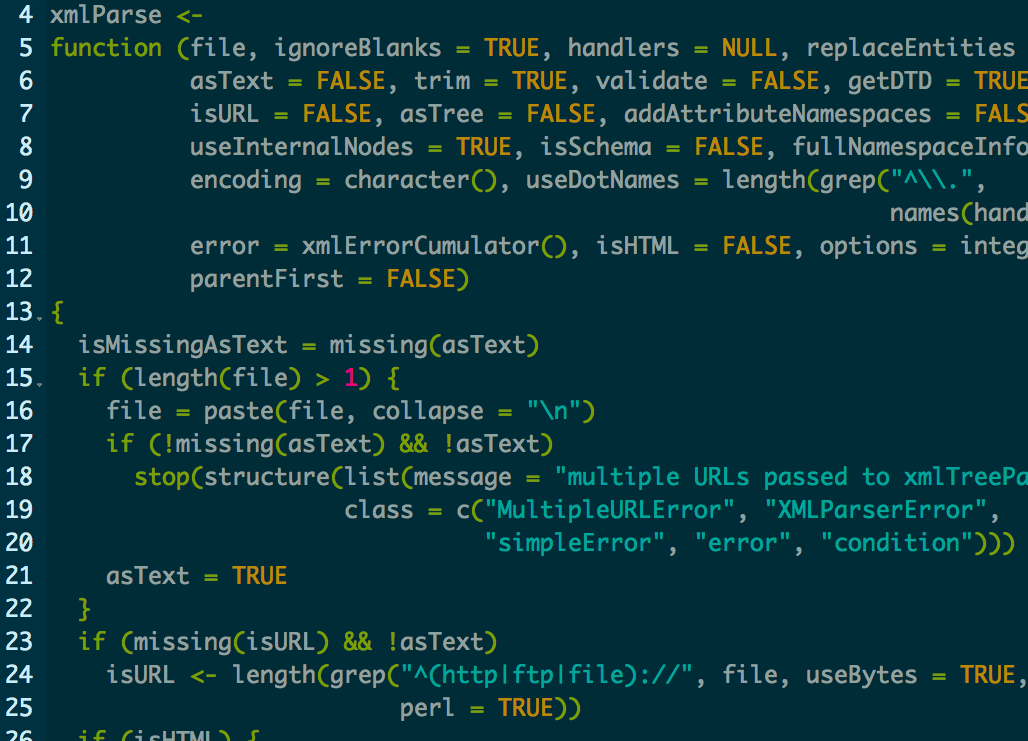
\includegraphics[width=\paperwidth]{images/xmlparsing_cover.png}
            };
        \end{tikzpicture}
     \end{frame}
}

%------------------------------------------------

\begin{frame}[fragile]
\frametitle{Readme}

\begin{block}{\scriptsize License:}
\tiny
 \begin{itemize}
  \item[] Creative Commons Attribution-NonCommercial-ShareAlike 4.0 International License \\ 
  \url{http://creativecommons.org/licenses/by-nc-sa/4.0/}{}
 \end{itemize}
\end{block}

\begin{block}{\scriptsize You are free to:}
\tiny
 \begin{itemize}
  \item[] \textcolor{darkgray}{\textbf{Share}} --- \textcolor{gray}{copy and redistribute the material}
  \item[] \textcolor{darkgray}{\textbf{Adapt}} --- \textcolor{gray}{rebuild and transform the material}
 \end{itemize}
\end{block}

\vspace{2mm}
\begin{block}{\scriptsize Under the following conditions:}
\tiny
\begin{itemize}
 \item[] \textcolor{darkgray}{\textbf{Attribution}} --- \textcolor{gray}{You must give appropriate credit, provide a link to the license, and indicate if changes were made.}
 \item[] \textcolor{darkgray}{\textbf{NonCommercial}} --- \textcolor{gray}{You may not use this work for commercial purposes.}
 \item[] \textcolor{darkgray}{\textbf{Share Alike}} --- \textcolor{gray}{If you remix, transform, or build upon this 
 work, you must distribute your contributions under the same license to this one.}
\end{itemize}
\end{block}

\end{frame}

%------------------------------------------------

\begin{frame}
\frametitle{Lectures Menu}

\begin{columns}[t]
\begin{column}{0.1\textwidth}
%--- empty space ---%
\end{column}
\begin{column}{0.8\textwidth}
 \begin{block}{Slide Decks}
  \begin{enumerate}
   \item \textcolor{lightgray}{Introduction}
   \item \textcolor{lightgray}{Reading files from the Web}
   \item \textcolor{lightgray}{Basics of XML and HTML}
   \item \textbf{Parsing XML / HTML content}
   \item \textcolor{lightgray}{Handling JSON data}
   \item \textcolor{lightgray}{HTTP Basics and the RCurl Package}   
   \item \textcolor{lightgray}{Getting data via web forms}
   \item \textcolor{lightgray}{Getting data via web services}
   %\item \textcolor{lightgray}{Web Scraping Case Study}
  \end{enumerate}
 \end{block}
\end{column}
\begin{column}{0.1\textwidth}
%--- empty space ---%
\end{column}
\end{columns}

\end{frame}

%------------------------------------------------

\begin{frame}
 \begin{center}
  \Huge{\textcolor{mandarina}{Parsing XML \\ and HTML Content}}
 \end{center}
\end{frame}

%------------------------------------------------

\begin{frame}
\frametitle{Goal}

\begin{columns}[t]
\begin{column}{0.1\textwidth}
%--- empty space ---%
\end{column}
\begin{column}{0.8\textwidth}

\begin{block}{Parsing XML / HTML docs}
The goal of these slides is to describe \textbf{how we can parse XML / HTML content} with the R package \highcode{"XML"}
\end{block}

\end{column}
\begin{column}{0.1\textwidth}
%--- empty space ---%
\end{column}
\end{columns}

\end{frame}

%------------------------------------------------

\begin{frame}
\frametitle{Synopsis}

\begin{columns}[t]
\begin{column}{0.1\textwidth}
%--- empty space ---%
\end{column}
\begin{column}{0.8\textwidth}

\begin{block}{In a nutshell}
We'll cover a variety of situations you most likely will find yourself dealing with:
\begin{itemize}
 \item R package XML
 \item Navigating the xml tree structure
 \item Main functions in package XML
 \item XPath
\end{itemize}
\end{block}

\end{column}
\begin{column}{0.1\textwidth}
%--- empty space ---%
\end{column}
\end{columns}

\end{frame}

%------------------------------------------------

\begin{frame}
\frametitle{Some References}

\begin{itemize}
 \item An Introduction to the XML Package for R \\
{\scriptsize \url{http://www.omegahat.org/RSXML/Tour.pdf}}
 \item A Short Introduction to the XML package for R \\
{\scriptsize \url{http://www.omegahat.org/RSXML/shortIntro.pdf}}
 \item R and Splus XML Parsers \\
 {\scriptsize \url{http://www.omegahat.org/RSXML/Overview.html}}
 \item XML and Web Technlogies for Data Sciences with R \\
 \low{by Deb Nolan and Duncan Temple Lang}
\end{itemize}

\end{frame}

%------------------------------------------------

\begin{frame}
\frametitle{Parsing}

\begin{quotation}
``A parser is a software component that takes input data (frequently text) and builds a data structure ---often some kind of parse tree, abstract syntax tree or other hierarchical structure--- giving a structural representation of the input, checking for correct syntax in the process''
\end{quotation}

{\footnotesize 
\hspace{8mm} \url{http://en.wikipedia.org/wiki/Parsing\#Parser} \\
}

\end{frame}

%------------------------------------------------

\begin{frame}
\frametitle{Parsing XML and HTML Content}

\begin{block}{Parsing XML and HTML?}
Getting data from the web often involves reading and processing content from xml and html documents. This is known as parsing. 

\bigskip
Luckily for us there's the R package \highcode{"XML"} \low{(by Duncan Temple Lang)} that allows us to parse such types of documents.
\end{block}

\end{frame}

%------------------------------------------------

\begin{frame}
 \begin{center}
  {\Huge \textcolor{mandarina}{R package \code{"XML"}}}
 \end{center}
\end{frame}

%------------------------------------------------

{ % all template changes are local to this group.
    \setbeamertemplate{navigation symbols}{}
    \begin{frame}[plain]
        \begin{tikzpicture}[remember picture,overlay]
            \node[at=(current page.center)] {
                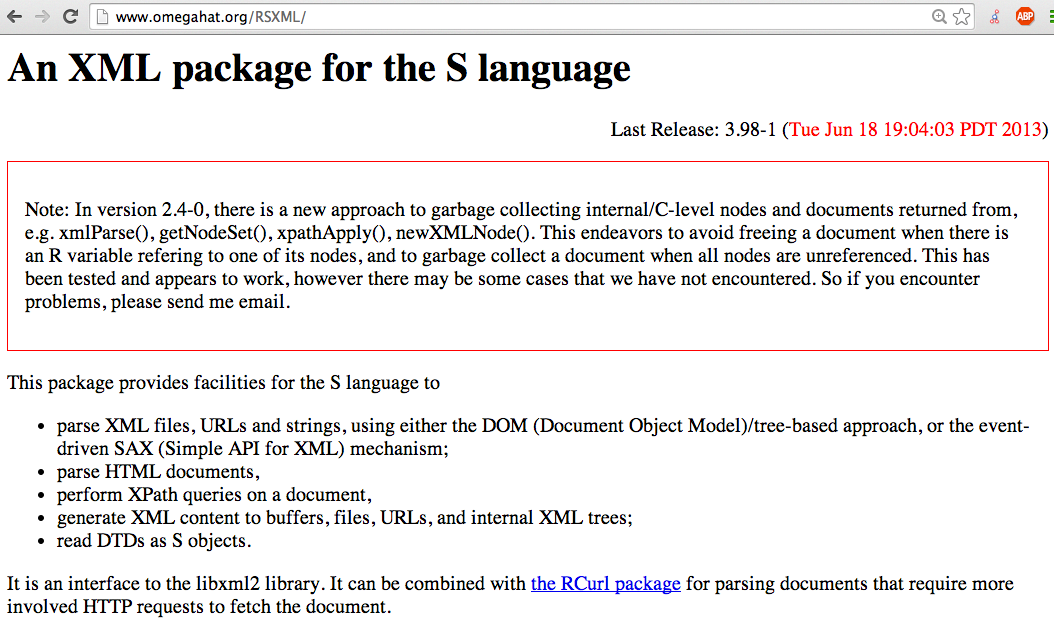
\includegraphics[width=\paperwidth]{images/xml_package.png}
            };
        \end{tikzpicture}
     \end{frame}
}

%------------------------------------------------

\begin{frame}
\frametitle{R Package XML}

The package \highcode{"XML"} is designed for 2 major purposes
\begin{enumerate}
 \item parsing xml / html content
 \item writing xml / html content
\end{enumerate}

\bigskip

\low{We won't cover the functions and utilities that have to do with writing xml / html content}

\end{frame}

%------------------------------------------------

\begin{frame}
\frametitle{What can we do with "XML"?}

We'll cover 4 major types of tasks that we can perform with \highcode{"XML"}
\begin{enumerate}
 \item parsing (ie \textit{reading}) xml / html content
 \item obtaining descriptive information about parsed contents
 \item navigating the tree structure \low{(ie accessing its components)}
 \item querying and extracting data from parsed contents
\end{enumerate}

\end{frame}

%------------------------------------------------

\begin{frame}[fragile]
\frametitle{Using \code{"XML"}}

If you don't have \code{"XML"} you'll need to install it first
\begin{knitrout}\tiny
\definecolor{shadecolor}{rgb}{1, 1, 1}\color{fgcolor}\begin{kframe}
\begin{alltt}
\hlcom{# installing xml}
\hlkwd{install.packages}\hlstd{(}\hlstr{"xml"}\hlstd{,} \hlkwc{dependencies} \hlstd{=} \hlnum{TRUE}\hlstd{)}
\end{alltt}
\end{kframe}
\end{knitrout}

Once installed it can be loaded
\begin{knitrout}\tiny
\definecolor{shadecolor}{rgb}{1, 1, 1}\color{fgcolor}\begin{kframe}
\begin{alltt}
\hlcom{# load XML}
\hlkwd{library}\hlstd{(XML)}
\end{alltt}
\end{kframe}
\end{knitrout}

More info about \code{"XML"} at: \\
{\scriptsize \url{http://www.omegahat.org/RSXML}}

\end{frame}

%------------------------------------------------

\begin{frame}
 \begin{center}
  {\Huge \textcolor{mandarina}{Parsing Functions}}
 \end{center}
\end{frame}

%------------------------------------------------

\begin{frame}
\frametitle{Function \code{xmlParse()}}

\begin{block}{Function \code{xmlParse()}}
\begin{itemize}
\item \code{"XML"} comes with the \textit{almighty} parser function \highcode{xmlParse()}
 \item the main input for \highcode{xmlParse()} is a file: either a local file, a complete URL or a text string
 \begin{itemize}
 \item[ex1:] \code{xmlParse("Documents/file.xml")}
 \item[ex2:] \code{xmlParse("http://www.xyz.com/some\_file.xml")}
 \item[ex3:] \code{xmlParse(xml\_string, asText=TRUE)}
 \end{itemize}
 \item the rest of the 20+ parameters are optional, and provide options to control the parsing procedure
\end{itemize}
\end{block}

\end{frame}

%------------------------------------------------

\begin{frame}[fragile]
\frametitle{\code{xmlParse()} default behavior}

\begin{block}{What does \code{xmlParse()} do?}
First let's talk about the \textbf{default behavior} of \highcode{xmlParse()} 
\begin{itemize}
 \item it is a DOM parser: it reads an XML document into a hierarchical structure representation
 \item it builds an XML tree as a native C-level data structure \\
 \low{(not an R data structure)}
 \item it returns an object of class \highcode{"XMLInternalDocument"}
 \item can read content from compressed files without us needing to explicitly uncompress the file
 \item it does NOT handle \code{HTTPS} \low{(secured HTTP)}
\end{itemize}
\end{block}

\end{frame}

%------------------------------------------------

\begin{frame}[fragile]
\frametitle{About \code{xmlParse()} (con't)}

\begin{block}{Default behavior}
Simple usage of \highcode{xmlParse()} on an XML document:
\begin{knitrout}\tiny
\definecolor{shadecolor}{rgb}{1, 1, 1}\color{fgcolor}\begin{kframe}
\begin{alltt}
\hlcom{# parsing an xml document}
\hlstd{doc1} \hlkwb{=} \hlkwd{xmlParse}\hlstd{(}\hlstr{"http://www.xmlfiles.com/examples/plant_catalog.xml"}\hlstd{)}
\end{alltt}
\end{kframe}
\end{knitrout}

\highcode{xmlParse()} returns an object of class \highcode{"XMLInternalDocument"} which is a C-level internal data structure

\begin{knitrout}\tiny
\definecolor{shadecolor}{rgb}{1, 1, 1}\color{fgcolor}\begin{kframe}
\begin{alltt}
\hlcom{# class }
\hlkwd{class}\hlstd{(doc1)}
\end{alltt}
\begin{verbatim}
## [1] "XMLInternalDocument" "XMLAbstractDocument"
\end{verbatim}
\end{kframe}
\end{knitrout}
\end{block}

\end{frame}

%------------------------------------------------

\begin{frame}[fragile]
\frametitle{About \code{xmlParse()} (con't)}

\begin{block}{Argument \code{useInternalNodes = FALSE}}
Instead of parsing content as an internal C-level structure, we can parse it into an R structure by specifying the parameter \highcode{useInternalNodes = FALSE}

\begin{knitrout}\tiny
\definecolor{shadecolor}{rgb}{1, 1, 1}\color{fgcolor}\begin{kframe}
\begin{alltt}
\hlcom{# parsing an xml document into an R structure}
\hlstd{doc2} \hlkwb{=} \hlkwd{xmlParse}\hlstd{(}\hlstr{"http://www.xmlfiles.com/examples/plant_catalog.xml"}\hlstd{,}
                \hlkwc{useInternalNodes} \hlstd{=} \hlnum{FALSE}\hlstd{)}
\end{alltt}
\end{kframe}
\end{knitrout}

the output is of class \highcode{"XMLDocument"} and is implemented as a hierarchy of lists

\begin{knitrout}\tiny
\definecolor{shadecolor}{rgb}{1, 1, 1}\color{fgcolor}\begin{kframe}
\begin{alltt}
\hlcom{# class }
\hlkwd{class}\hlstd{(doc2)}
\end{alltt}
\begin{verbatim}
## [1] "XMLDocument"         "XMLAbstractDocument"
\end{verbatim}
\begin{alltt}
\hlkwd{is.list}\hlstd{(doc2)}
\end{alltt}
\begin{verbatim}
## [1] TRUE
\end{verbatim}
\end{kframe}
\end{knitrout}
\end{block}

\end{frame}

%------------------------------------------------

\begin{frame}[fragile]
\frametitle{About \code{xmlTreeParse()}}

\begin{block}{Argument \code{useInternalNodes = FALSE}}
\code{"XML"} provides the function \highcode{xmlTreeParse()} as a convenient synonym for \code{xmlParse(file, useInternalNodes = FALSE)}

\begin{knitrout}\tiny
\definecolor{shadecolor}{rgb}{1, 1, 1}\color{fgcolor}\begin{kframe}
\begin{alltt}
\hlcom{# parse an xml document into an R structure}
\hlstd{doc3} \hlkwb{=} \hlkwd{xmlTreeParse}\hlstd{(}\hlstr{"http://www.xmlfiles.com/examples/plant_catalog.xml"}\hlstd{)}
\end{alltt}
\end{kframe}
\end{knitrout}

As expected, the output is of class \highcode{"XMLDocument"}

\begin{knitrout}\tiny
\definecolor{shadecolor}{rgb}{1, 1, 1}\color{fgcolor}\begin{kframe}
\begin{alltt}
\hlcom{# class }
\hlkwd{class}\hlstd{(doc3)}
\end{alltt}
\begin{verbatim}
## [1] "XMLDocument"         "XMLAbstractDocument"
\end{verbatim}
\begin{alltt}
\hlkwd{identical}\hlstd{(doc2, doc3)}
\end{alltt}
\begin{verbatim}
## [1] TRUE
\end{verbatim}
\end{kframe}
\end{knitrout}

\end{block}

\end{frame}

%------------------------------------------------

\begin{frame}[fragile]
\frametitle{HTML Content}

\begin{block}{Parsing HTML content}
In theory, we could use \highcode{xmlParse()} with its default settings to parse HTML documents. 

\bigskip
However \code{xmlParse()} ---with its default behavior--- will not work properly when HTML documents are not well-formed:
\begin{itemize}
 \item no xml declaration
 \item no DOCTYPE
 \item no closure of tags
\end{itemize}
\end{block}

\end{frame}

%------------------------------------------------

\begin{frame}[fragile]
\frametitle{\code{xmlParse()} and HTML Content}

\begin{block}{Argument \code{isHTML = TRUE}}
One option to parse HTML documents is by using \code{xmlParse()} with the argument \highcode{isHTML = TRUE}

\begin{knitrout}\tiny
\definecolor{shadecolor}{rgb}{1, 1, 1}\color{fgcolor}\begin{kframe}
\begin{alltt}
\hlcom{# parsing an html document with 'xmlParse()'}
\hlstd{doc4} \hlkwb{=} \hlkwd{xmlParse}\hlstd{(}\hlstr{"http://www.r-project.org/mail.html"}\hlstd{,}
                \hlkwc{isHTML} \hlstd{=} \hlnum{TRUE}\hlstd{)}
\end{alltt}
\end{kframe}
\end{knitrout}

the output is of class \highcode{"HTMLInternalDocument"}



\begin{knitrout}\tiny
\definecolor{shadecolor}{rgb}{1, 1, 1}\color{fgcolor}\begin{kframe}
\begin{alltt}
\hlcom{# class }
\hlkwd{class}\hlstd{(doc4)}
\end{alltt}
\begin{verbatim}
## [1] "HTMLInternalDocument" "HTMLInternalDocument" "XMLInternalDocument" 
## [4] "XMLAbstractDocument"
\end{verbatim}
\end{kframe}
\end{knitrout}
\end{block}

\end{frame}

%------------------------------------------------

\begin{frame}[fragile]
\frametitle{\code{htmlParse()} and HTML Content}

\begin{block}{Function \code{htmlParse()}}
Another option is to use the function \highcode{htmlParse()} which is equivalent to \code{xmlParse(file, isHTML = TRUE)}

\begin{knitrout}\tiny
\definecolor{shadecolor}{rgb}{1, 1, 1}\color{fgcolor}\begin{kframe}
\begin{alltt}
\hlcom{# parsing an html document with 'htmlParse()'}
\hlstd{doc5} \hlkwb{=} \hlkwd{htmlParse}\hlstd{(}\hlstr{"http://www.r-project.org/mail.html"}\hlstd{)}
\end{alltt}
\end{kframe}
\end{knitrout}

again, the output is of class \highcode{"HTMLInternalDocument"}

\begin{knitrout}\tiny
\definecolor{shadecolor}{rgb}{1, 1, 1}\color{fgcolor}\begin{kframe}
\begin{alltt}
\hlcom{# class }
\hlkwd{class}\hlstd{(doc5)}
\end{alltt}
\begin{verbatim}
## [1] "HTMLInternalDocument" "HTMLInternalDocument" "XMLInternalDocument" 
## [4] "XMLAbstractDocument"
\end{verbatim}
\end{kframe}
\end{knitrout}
\end{block}

\end{frame}

%------------------------------------------------

\begin{frame}[fragile]
\frametitle{Function \code{htmlTreeParse()}}

\begin{block}{Function \code{htmlTreeParse()}}
To parse content into an R structure we have to use \highcode{htmlTreeParse()} which is equivalent to \code{htmlParse(file, useInternalNodes = FALSE)}

\begin{knitrout}\tiny
\definecolor{shadecolor}{rgb}{1, 1, 1}\color{fgcolor}\begin{kframe}
\begin{alltt}
\hlcom{# parsing an html document into an  R structure}
\hlstd{doc6} \hlkwb{=} \hlkwd{htmlTreeParse}\hlstd{(}\hlstr{"http://www.r-project.org/mail.html"}\hlstd{)}
\end{alltt}
\end{kframe}
\end{knitrout}

in this case the output is of class \highcode{"XMLDocumentContent"}

\begin{knitrout}\tiny
\definecolor{shadecolor}{rgb}{1, 1, 1}\color{fgcolor}\begin{kframe}
\begin{alltt}
\hlcom{# class }
\hlkwd{class}\hlstd{(doc6)}
\end{alltt}
\begin{verbatim}
## [1] "XMLDocumentContent"
\end{verbatim}
\end{kframe}
\end{knitrout}
\end{block}

\end{frame}

%------------------------------------------------

\begin{frame}[fragile]
\frametitle{HTML Content}

\begin{block}{About parsing HTML documents}
\begin{itemize}
 \item \code{xmlParse()} can do the job but only on well-formed HTML
 \item it is better to be conservative and use the argument \highcode{isHTML = TRUE}, which is equivalent to using \code{htmlParse()}
 \item we can use \highcode{htmlParse()} or \highcode{htmlTreeParse()} which try to correct not well-formed docs by using heuristics that will take care of the missing elements
 \item in a worst-case scenario we can use \highcode{tidyHTML()} from the R package \code{"RTidyHTML"}, and then pass the result to \code{htmlParse()}
\end{itemize}
\end{block}

\end{frame}

%------------------------------------------------

\begin{frame}[fragile]
\frametitle{Parsing Functions Summary}

\begin{block}{\code{xmlParse(file)}}
\begin{itemize}
 \item main parsing function
 \item returns class \code{"XMLInternalDocument"} \low{(C-level structure)}
\end{itemize}
\end{block}

\begin{block}{\code{xmlTreeParse(file)}}
\begin{itemize}
 \item returns class \code{"XMLDocument"} \low{(R data structure)}
 \item equivalent to \code{xmlParse(file, useInternalNodes = FALSE)}
\end{itemize}
\end{block}

\end{frame}

%------------------------------------------------

\begin{frame}[fragile]
\frametitle{Parsing Functions Summary}

\begin{block}{\code{htmlParse(file)}}
\begin{itemize}
 \item especially suited for parsing HTML content
 \item returns class \code{"HTMLInternalDocument"} \low{(C-level structure)}
 \item equivalent to \code{xmlParse(file, isHTML = TRUE)}
\end{itemize}
\end{block}

\begin{block}{\code{htmlTreeParse(file)}}
\begin{itemize}
 \item especially suited for parsing HTML content
 \item returns class \code{"XMLDocumentContent"} \low{(R data structure)}
 \item equivalent to
 \begin{itemize}
  \item \code{xmlParse(file, isHTML = TRUE, useInternalNodes = FALSE)}
  \item \code{htmlParse(file, useInternalNodes = FALSE)}
 \end{itemize}
\end{itemize}
\end{block}

\end{frame}

%------------------------------------------------

\begin{frame}
 \begin{center}
  {\Huge \textcolor{mandarina}{Working with \\ Parsed Documents}}
 \end{center}
\end{frame}

%------------------------------------------------

\begin{frame}
\frametitle{Parsed Documents}

\begin{block}{\code{xmlRoot()} and \code{xmlChildren()}}
Having parsed an XML / HTML document, we can use 2 main functions to start working on the tree structure:
\begin{itemize}
 \item \highcode{xmlRoot()} gets access to the root node and its elements 
 \item \highcode{xmlChildren()} gets access to the child elements of a given node
\end{itemize}
\end{block}

\end{frame}

%------------------------------------------------

\begin{frame}[fragile]
\frametitle{Conceptual Diagram}

\begin{center}
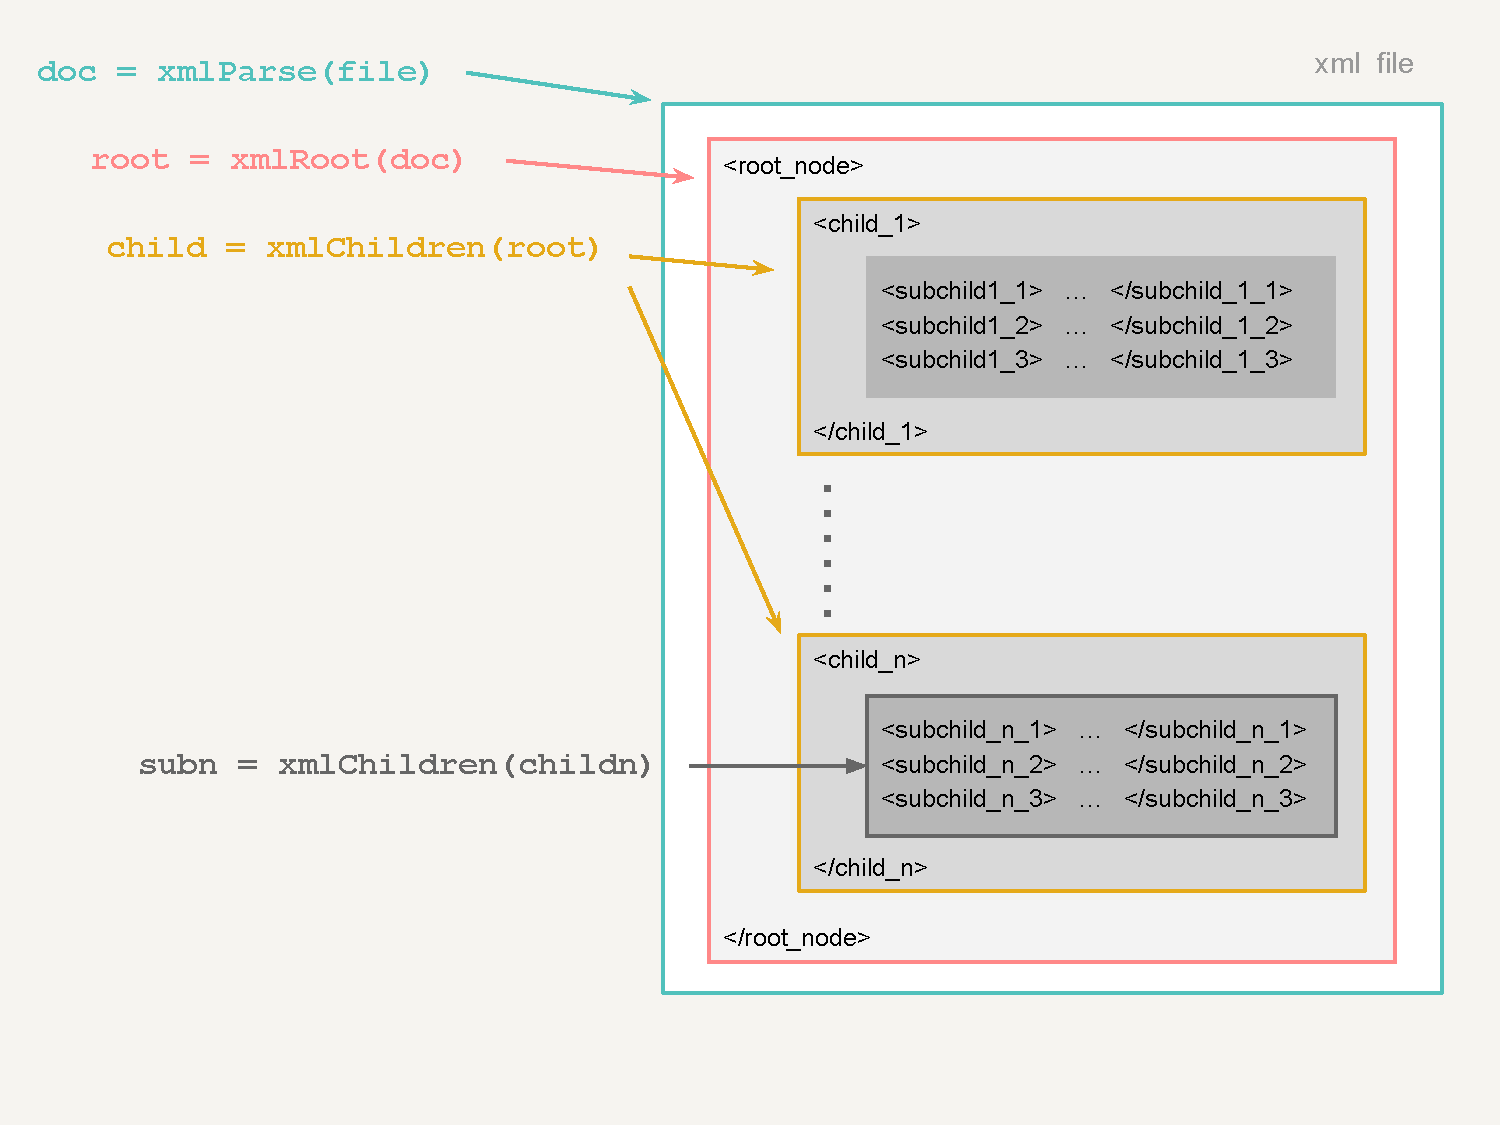
\includegraphics[width=11cm]{images/xml_tree_navigate.pdf}
\end{center}

\end{frame}

%------------------------------------------------

\begin{frame}
\frametitle{Some Additional Functions}

\begin{center}
\textcolor{turquoise}{Functions for a given node}
\end{center}

\begin{center}
 \begin{tabular}{l l}
  \hline
  Function & Description \\
  \hline
  \code{xmlName()} & name of the node \\
  \code{xmlSize()} & number of subnodes \\
  \code{xmlAttrs()} & named character vector of all attributes \\
  \code{xmlGetAttr()} & value of a single attribute \\
  \code{xmlValue()} & contents of a leaf node \\
  \code{xmlParent()} & name of parent node \\
  \code{xmlAncestors()} & name of ancestor nodes \\
  \code{getSibling()} & siblings to the right or to the left \\
  \code{xmlNamespace()} & the namespace (if there's one) \\  
  \hline
 \end{tabular}
\end{center}

{\scriptsize \low{The applicability of the functions depends on the class of objects we are working on}}

\end{frame}

%------------------------------------------------

\begin{frame}[fragile]
\frametitle{Toy Example: Movies XML}

\begin{columns}[t]
\begin{column}{0.5\textwidth}
\begin{knitrout}\tiny
\definecolor{shadecolor}{rgb}{1, 1, 1}\color{fgcolor}\begin{kframe}
\begin{alltt}
\hlcom{# define some xml content}
\hlstd{xml_string} \hlkwb{=} \hlkwd{c}\hlstd{(}
  \hlstr{'<?xml version="1.0" encoding="UTF-8"?>'}\hlstd{,}
  \hlstr{'<movies>'}\hlstd{,}
  \hlstr{'<movie mins="126" lang="eng">'}\hlstd{,}
  \hlstr{'<title>Good Will Hunting</title>'}\hlstd{,}
  \hlstr{'<director>'}\hlstd{,}
  \hlstr{'<first_name>Gus</first_name>'}\hlstd{,}
  \hlstr{'<last_name>Van Sant</last_name>'}\hlstd{,}
  \hlstr{'</director>'}\hlstd{,}
  \hlstr{'<year>1998</year>'}\hlstd{,}
  \hlstr{'<genre>drama</genre>'}\hlstd{,}
  \hlstr{'</movie>'}\hlstd{,}
  \hlstr{'<movie mins="106" lang="spa">'}\hlstd{,}
  \hlstr{'<title>Y tu mama tambien</title>'}\hlstd{,}
  \hlstr{'<director>'}\hlstd{,}
  \hlstr{'<first_name>Alfonso</first_name>'}\hlstd{,}
  \hlstr{'<last_name>Cuaron</last_name>'}\hlstd{,}
  \hlstr{'</director>'}\hlstd{,}
  \hlstr{'<year>2001</year>'}\hlstd{,}
  \hlstr{'<genre>drama</genre>'}\hlstd{,}
  \hlstr{'</movie>'}\hlstd{,}
  \hlstr{'</movies>'}\hlstd{)}

\hlcom{# parse xml content}
\hlstd{movies_xml} \hlkwb{=} \hlkwd{xmlParse}\hlstd{(xml_string,} \hlkwc{asText} \hlstd{=} \hlnum{TRUE}\hlstd{)}
\end{alltt}
\end{kframe}
\end{knitrout}
\end{column}

\begin{column}{0.5\textwidth}
\begin{knitrout}\tiny
\definecolor{shadecolor}{rgb}{1, 1, 1}\color{fgcolor}\begin{kframe}
\begin{alltt}
\hlcom{# check movies_xml}
\hlstd{movies_xml}
\end{alltt}
\begin{verbatim}
## <?xml version="1.0" encoding="UTF-8"?>
## <movies>
##   <movie mins="126" lang="eng">
##     <title>Good Will Hunting</title>
##     <director>
##       <first_name>Gus</first_name>
##       <last_name>Van Sant</last_name>
##     </director>
##     <year>1998</year>
##     <genre>drama</genre>
##   </movie>
##   <movie mins="106" lang="spa">
##     <title>Y tu mama tambien</title>
##     <director>
##       <first_name>Alfonso</first_name>
##       <last_name>Cuaron</last_name>
##     </director>
##     <year>2001</year>
##     <genre>drama</genre>
##   </movie>
## </movies>
## 
\end{verbatim}
\end{kframe}
\end{knitrout}
\end{column}
\end{columns}

\end{frame}

%------------------------------------------------

\begin{frame}[fragile]
\frametitle{Movies XML: Root Node}

\begin{columns}[t]
\begin{column}{0.5\textwidth}
\begin{knitrout}\tiny
\definecolor{shadecolor}{rgb}{1, 1, 1}\color{fgcolor}\begin{kframe}
\begin{alltt}
\hlcom{# examine class}
\hlcom{# (movies_xml is a C-level object)}
\hlkwd{class}\hlstd{(movies_xml)}
\end{alltt}
\begin{verbatim}
## [1] "XMLInternalDocument" "XMLAbstractDocument"
\end{verbatim}
\begin{alltt}
\hlcom{# get root node}
\hlstd{root} \hlkwb{=} \hlkwd{xmlRoot}\hlstd{(movies_xml)}

\hlcom{# examine class}
\hlkwd{class}\hlstd{(root)}
\end{alltt}
\begin{verbatim}
## [1] "XMLInternalElementNode" "XMLInternalNode"        "XMLAbstractNode"
\end{verbatim}
\end{kframe}
\end{knitrout}
\end{column}

\begin{column}{0.5\textwidth}
\begin{knitrout}\tiny
\definecolor{shadecolor}{rgb}{1, 1, 1}\color{fgcolor}\begin{kframe}
\begin{alltt}
\hlcom{# display root node}
\hlstd{root}
\end{alltt}
\begin{verbatim}
## <movies>
##   <movie mins="126" lang="eng">
##     <title>Good Will Hunting</title>
##     <director>
##       <first_name>Gus</first_name>
##       <last_name>Van Sant</last_name>
##     </director>
##     <year>1998</year>
##     <genre>drama</genre>
##   </movie>
##   <movie mins="106" lang="spa">
##     <title>Y tu mama tambien</title>
##     <director>
##       <first_name>Alfonso</first_name>
##       <last_name>Cuaron</last_name>
##     </director>
##     <year>2001</year>
##     <genre>drama</genre>
##   </movie>
## </movies>
\end{verbatim}
\end{kframe}
\end{knitrout}
\end{column}
\end{columns}

\end{frame}

%------------------------------------------------

\begin{frame}[fragile]
\frametitle{Movies XML: movie children}

\begin{columns}[t]
\begin{column}{0.5\textwidth}
\begin{knitrout}\tiny
\definecolor{shadecolor}{rgb}{1, 1, 1}\color{fgcolor}\begin{kframe}
\begin{alltt}
\hlcom{# children of root node}
\hlstd{movie_child} \hlkwb{=} \hlkwd{xmlChildren}\hlstd{(root)}

\hlstd{movie_child}
\end{alltt}
\begin{verbatim}
## $movie
## <movie mins="126" lang="eng">
##   <title>Good Will Hunting</title>
##   <director>
##     <first_name>Gus</first_name>
##     <last_name>Van Sant</last_name>
##   </director>
##   <year>1998</year>
##   <genre>drama</genre>
## </movie> 
## 
## $movie
## <movie mins="106" lang="spa">
##   <title>Y tu mama tambien</title>
##   <director>
##     <first_name>Alfonso</first_name>
##     <last_name>Cuaron</last_name>
##   </director>
##   <year>2001</year>
##   <genre>drama</genre>
## </movie> 
## 
## attr(,"class")
## [1] "XMLInternalNodeList" "XMLNodeList"
\end{verbatim}
\end{kframe}
\end{knitrout}
\end{column}

\begin{column}{0.5\textwidth}
\begin{knitrout}\tiny
\definecolor{shadecolor}{rgb}{1, 1, 1}\color{fgcolor}\begin{kframe}
\begin{alltt}
\hlcom{# first movie}
\hlstd{goodwill} \hlkwb{=} \hlstd{movie_child[[}\hlnum{1}\hlstd{]]}
\hlstd{goodwill}
\end{alltt}
\begin{verbatim}
## <movie mins="126" lang="eng">
##   <title>Good Will Hunting</title>
##   <director>
##     <first_name>Gus</first_name>
##     <last_name>Van Sant</last_name>
##   </director>
##   <year>1998</year>
##   <genre>drama</genre>
## </movie>
\end{verbatim}
\begin{alltt}
\hlcom{# second movie}
\hlstd{tumama} \hlkwb{=} \hlstd{movie_child[[}\hlnum{2}\hlstd{]]}
\hlstd{tumama}
\end{alltt}
\begin{verbatim}
## <movie mins="106" lang="spa">
##   <title>Y tu mama tambien</title>
##   <director>
##     <first_name>Alfonso</first_name>
##     <last_name>Cuaron</last_name>
##   </director>
##   <year>2001</year>
##   <genre>drama</genre>
## </movie>
\end{verbatim}
\end{kframe}
\end{knitrout}
\end{column}
\end{columns}

\end{frame}

%------------------------------------------------

\begin{frame}[fragile]
\frametitle{Movies XML: movie children}

\begin{columns}[t]
\begin{column}{0.5\textwidth}
\begin{knitrout}\tiny
\definecolor{shadecolor}{rgb}{1, 1, 1}\color{fgcolor}\begin{kframe}
\begin{alltt}
\hlcom{# node name}
\hlkwd{xmlName}\hlstd{(goodwill)}
\end{alltt}
\begin{verbatim}
## [1] "movie"
\end{verbatim}
\begin{alltt}
\hlcom{# number of children}
\hlkwd{xmlSize}\hlstd{(goodwill)}
\end{alltt}
\begin{verbatim}
## [1] 4
\end{verbatim}
\begin{alltt}
\hlcom{# node attributes}
\hlkwd{xmlAttrs}\hlstd{(goodwill)}
\end{alltt}
\begin{verbatim}
##  mins  lang 
## "126" "eng"
\end{verbatim}
\begin{alltt}
\hlcom{# get specific attribute value}
\hlkwd{xmlGetAttr}\hlstd{(goodwill,} \hlkwc{name} \hlstd{=} \hlstr{'lang'}\hlstd{)}
\end{alltt}
\begin{verbatim}
## [1] "eng"
\end{verbatim}
\end{kframe}
\end{knitrout}
\end{column}

\begin{column}{0.5\textwidth}
\begin{knitrout}\tiny
\definecolor{shadecolor}{rgb}{1, 1, 1}\color{fgcolor}\begin{kframe}
\begin{alltt}
\hlcom{# node name}
\hlkwd{xmlName}\hlstd{(tumama)}
\end{alltt}
\begin{verbatim}
## [1] "movie"
\end{verbatim}
\begin{alltt}
\hlcom{# number of children}
\hlkwd{xmlSize}\hlstd{(tumama)}
\end{alltt}
\begin{verbatim}
## [1] 4
\end{verbatim}
\begin{alltt}
\hlcom{# node attributes}
\hlkwd{xmlAttrs}\hlstd{(tumama)}
\end{alltt}
\begin{verbatim}
##  mins  lang 
## "106" "spa"
\end{verbatim}
\begin{alltt}
\hlcom{# get specific attribute value}
\hlkwd{xmlGetAttr}\hlstd{(tumama,} \hlkwc{name} \hlstd{=} \hlstr{'lang'}\hlstd{)}
\end{alltt}
\begin{verbatim}
## [1] "spa"
\end{verbatim}
\end{kframe}
\end{knitrout}
\end{column}
\end{columns}

\end{frame}

%------------------------------------------------

\begin{frame}[fragile]
\frametitle{Movies XML: movie Good Will Hunting}

\begin{columns}[t]
\begin{column}{0.5\textwidth}
\begin{knitrout}\tiny
\definecolor{shadecolor}{rgb}{1, 1, 1}\color{fgcolor}\begin{kframe}
\begin{alltt}
\hlcom{# node content (as character string)}
\hlkwd{xmlValue}\hlstd{(goodwill)}
\end{alltt}
\begin{verbatim}
## [1] "Good Will HuntingGusVan Sant1998drama"
\end{verbatim}
\begin{alltt}
\hlcom{# child nodes of goodwill node}
\hlkwd{xmlChildren}\hlstd{(goodwill)}
\end{alltt}
\begin{verbatim}
## $title
## <title>Good Will Hunting</title> 
## 
## $director
## <director>
##   <first_name>Gus</first_name>
##   <last_name>Van Sant</last_name>
## </director> 
## 
## $year
## <year>1998</year> 
## 
## $genre
## <genre>drama</genre> 
## 
## attr(,"class")
## [1] "XMLInternalNodeList" "XMLNodeList"
\end{verbatim}
\end{kframe}
\end{knitrout}
\end{column}

\begin{column}{0.5\textwidth}
\begin{knitrout}\tiny
\definecolor{shadecolor}{rgb}{1, 1, 1}\color{fgcolor}\begin{kframe}
\begin{alltt}
\hlcom{# director nodes of goodwill node}
\hlstd{gusvan} \hlkwb{=} \hlkwd{xmlChildren}\hlstd{(goodwill)[[}\hlnum{2}\hlstd{]]}
\hlstd{gusvan}
\end{alltt}
\begin{verbatim}
## <director>
##   <first_name>Gus</first_name>
##   <last_name>Van Sant</last_name>
## </director>
\end{verbatim}
\begin{alltt}
\hlcom{# parent}
\hlkwd{xmlParent}\hlstd{(gusvan)}
\end{alltt}
\begin{verbatim}
## <movie mins="126" lang="eng">
##   <title>Good Will Hunting</title>
##   <director>
##     <first_name>Gus</first_name>
##     <last_name>Van Sant</last_name>
##   </director>
##   <year>1998</year>
##   <genre>drama</genre>
## </movie>
\end{verbatim}
\end{kframe}
\end{knitrout}
\end{column}
\end{columns}

\end{frame}

%------------------------------------------------

\begin{frame}[fragile]
\frametitle{Movies XML: movie Good Will Hunting}

\begin{columns}[t]
\begin{column}{0.5\textwidth}
\begin{knitrout}\tiny
\definecolor{shadecolor}{rgb}{1, 1, 1}\color{fgcolor}\begin{kframe}
\begin{alltt}
\hlcom{# director children}
\hlkwd{xmlChildren}\hlstd{(gusvan)}
\end{alltt}
\begin{verbatim}
## $first_name
## <first_name>Gus</first_name> 
## 
## $last_name
## <last_name>Van Sant</last_name> 
## 
## attr(,"class")
## [1] "XMLInternalNodeList" "XMLNodeList"
\end{verbatim}
\end{kframe}
\end{knitrout}
\end{column}

\begin{column}{0.5\textwidth}
\begin{knitrout}\tiny
\definecolor{shadecolor}{rgb}{1, 1, 1}\color{fgcolor}\begin{kframe}
\begin{alltt}
\hlcom{# sibling of goodwill node}
\hlkwd{getSibling}\hlstd{(goodwill)}
\end{alltt}
\begin{verbatim}
## <movie mins="106" lang="spa">
##   <title>Y tu mama tambien</title>
##   <director>
##     <first_name>Alfonso</first_name>
##     <last_name>Cuaron</last_name>
##   </director>
##   <year>2001</year>
##   <genre>drama</genre>
## </movie>
\end{verbatim}
\end{kframe}
\end{knitrout}
\end{column}
\end{columns}

\end{frame}

%------------------------------------------------

\begin{frame}
 \begin{center}
  {\Huge \textcolor{mandarina}{Looping Over Nodes}}
 \end{center}
\end{frame}

%------------------------------------------------

\begin{frame}[fragile]
\frametitle{Looping Over Nodes}

\begin{block}{Looping over nodes}
Extracting data from an XML / HTML document involves applying a given function to a subset of nodes. This means iterating over such subset.

\bigskip
There are various ways to loop over a subset of nodes:
\begin{itemize}
 \item the most basic approach is with \highcode{sapply()} or \highcode{lapply()}
 \item anoter way is by using the ad-hoc functions \highcode{xmlApply()} and \highcode{xmlSApply()}, which are simple wrappers for the \code{lapply()} and \code{sapply()} functions. 
\end{itemize}
\end{block}

\end{frame}

%------------------------------------------------

\begin{frame}[fragile]
\frametitle{Looping Over Nodes}

Some iteration examples with \highcode{sapply()}

\begin{columns}[t]
\begin{column}{0.5\textwidth}
\begin{knitrout}\tiny
\definecolor{shadecolor}{rgb}{1, 1, 1}\color{fgcolor}\begin{kframe}
\begin{alltt}
\hlcom{# length}
\hlkwd{sapply}\hlstd{(movie_child, length)}
\end{alltt}
\begin{verbatim}
## movie movie 
##     1     1
\end{verbatim}
\begin{alltt}
\hlcom{# names in child nodes}
\hlkwd{sapply}\hlstd{(movie_child, names)}
\end{alltt}
\begin{verbatim}
##          movie      movie     
## title    "title"    "title"   
## director "director" "director"
## year     "year"     "year"    
## genre    "genre"    "genre"
\end{verbatim}
\begin{alltt}
\hlkwd{sapply}\hlstd{(movie_child, xmlSize)}
\end{alltt}
\begin{verbatim}
## movie movie 
##     4     4
\end{verbatim}
\end{kframe}
\end{knitrout}
\end{column}

\begin{column}{0.5\textwidth}
\begin{knitrout}\tiny
\definecolor{shadecolor}{rgb}{1, 1, 1}\color{fgcolor}\begin{kframe}
\begin{alltt}
\hlcom{# attributes of root child nodes}
\hlkwd{sapply}\hlstd{(movie_child, xmlAttrs)}
\end{alltt}
\begin{verbatim}
##      movie movie
## mins "126" "106"
## lang "eng" "spa"
\end{verbatim}
\begin{alltt}
\hlcom{# names in child nodes}
\hlkwd{sapply}\hlstd{(movie_child, xmlValue)}
\end{alltt}
\begin{verbatim}
##                                     movie 
##   "Good Will HuntingGusVan Sant1998drama" 
##                                     movie 
## "Y tu mama tambienAlfonsoCuaron2001drama"
\end{verbatim}
\end{kframe}
\end{knitrout}
\end{column}
\end{columns}

\end{frame}

%------------------------------------------------

\begin{frame}[fragile]
\frametitle{Looping Over Nodes}

\highcode{xmlApply()} and \highcode{xmlSApply()} operate on the sub-nodes of the XML node:

\begin{columns}[t]
\begin{column}{0.5\textwidth}
\begin{knitrout}\tiny
\definecolor{shadecolor}{rgb}{1, 1, 1}\color{fgcolor}\begin{kframe}
\begin{alltt}
\hlcom{# names in child nodes}
\hlkwd{xmlSApply}\hlstd{(root, names)}
\end{alltt}
\begin{verbatim}
##          movie      movie     
## title    "title"    "title"   
## director "director" "director"
## year     "year"     "year"    
## genre    "genre"    "genre"
\end{verbatim}
\begin{alltt}
\hlcom{# size of movie children}
\hlkwd{xmlSApply}\hlstd{(root, xmlSize)}
\end{alltt}
\begin{verbatim}
## movie movie 
##     4     4
\end{verbatim}
\end{kframe}
\end{knitrout}
\end{column}

\begin{column}{0.5\textwidth}
\begin{knitrout}\tiny
\definecolor{shadecolor}{rgb}{1, 1, 1}\color{fgcolor}\begin{kframe}
\begin{alltt}
\hlcom{# attributes of root child nodes}
\hlkwd{xmlSApply}\hlstd{(root, xmlAttrs)}
\end{alltt}
\begin{verbatim}
##      movie movie
## mins "126" "106"
## lang "eng" "spa"
\end{verbatim}
\begin{alltt}
\hlcom{# names in child nodes}
\hlkwd{xmlSApply}\hlstd{(root, xmlValue)}
\end{alltt}
\begin{verbatim}
##                                     movie 
##   "Good Will HuntingGusVan Sant1998drama" 
##                                     movie 
## "Y tu mama tambienAlfonsoCuaron2001drama"
\end{verbatim}
\end{kframe}
\end{knitrout}
\end{column}
\end{columns}

\end{frame}

%------------------------------------------------

\begin{frame}[fragile]
\frametitle{Looping Over Nodes}

\begin{columns}[t]
\begin{column}{0.5\textwidth}
\begin{knitrout}\tiny
\definecolor{shadecolor}{rgb}{1, 1, 1}\color{fgcolor}\begin{kframe}
\begin{alltt}
\hlcom{# length of nodes in movie 1}
\hlkwd{xmlSApply}\hlstd{(root[[}\hlnum{1}\hlstd{]], length)}
\end{alltt}
\begin{verbatim}
##    title director     year    genre 
##        1        1        1        1
\end{verbatim}
\begin{alltt}
\hlcom{# size in child nodes in movie 1}
\hlkwd{xmlSApply}\hlstd{(root[[}\hlnum{1}\hlstd{]], xmlSize)}
\end{alltt}
\begin{verbatim}
##    title director     year    genre 
##        1        2        1        1
\end{verbatim}
\begin{alltt}
\hlcom{# attribute values of nodes in movie 1}
\hlkwd{xmlSApply}\hlstd{(root[[}\hlnum{1}\hlstd{]], xmlValue)}
\end{alltt}
\begin{verbatim}
##               title            director                year 
## "Good Will Hunting"       "GusVan Sant"              "1998" 
##               genre 
##             "drama"
\end{verbatim}
\end{kframe}
\end{knitrout}
\end{column}

\begin{column}{0.5\textwidth}
\begin{knitrout}\tiny
\definecolor{shadecolor}{rgb}{1, 1, 1}\color{fgcolor}\begin{kframe}
\begin{alltt}
\hlcom{# length of nodes in movie 2}
\hlkwd{xmlSApply}\hlstd{(root[[}\hlnum{2}\hlstd{]], length)}
\end{alltt}
\begin{verbatim}
##    title director     year    genre 
##        1        1        1        1
\end{verbatim}
\begin{alltt}
\hlcom{# size in child nodes in movie 2}
\hlkwd{xmlSApply}\hlstd{(root[[}\hlnum{2}\hlstd{]], xmlSize)}
\end{alltt}
\begin{verbatim}
##    title director     year    genre 
##        1        2        1        1
\end{verbatim}
\begin{alltt}
\hlcom{# attribute values of nodes in movie 2}
\hlkwd{xmlSApply}\hlstd{(root[[}\hlnum{2}\hlstd{]], xmlValue)}
\end{alltt}
\begin{verbatim}
##               title            director                year 
## "Y tu mama tambien"     "AlfonsoCuaron"              "2001" 
##               genre 
##             "drama"
\end{verbatim}
\end{kframe}
\end{knitrout}
\end{column}
\end{columns}

\end{frame}

%------------------------------------------------

\begin{frame}
 \begin{center}
  {\Huge \textcolor{mandarina}{XPath Language}}
 \end{center}
\end{frame}

%------------------------------------------------

\begin{frame}
\frametitle{XPath}

\begin{columns}[t]
\begin{column}{0.1\textwidth}
%--- empty space ---%
\end{column}
\begin{column}{0.8\textwidth}

\begin{block}{Querying Trees}
The real parsing power comes from the ability to \textbf{locate nodes and extract information from them}. For this, we need to be able to perform queries on the parsed content.
\end{block}

\begin{block}{XPath}
The solution is provided by \textbf{XPath}, which is a language to navigate through elements and attributes in an XML/HTML document
\end{block}

\end{column}
\begin{column}{0.1\textwidth}
%--- empty space ---%
\end{column}
\end{columns}

\end{frame}

%------------------------------------------------

\begin{frame}
\frametitle{XPath}

\begin{block}{XPath}
\begin{itemize}
 \item is a language for finding information in an XML document
 \item uses path expressions to select nodes or node-sets in an XML document
 \item works by identifying patterns to match data or content
 \item includes over 100 built-in functions
\end{itemize}
\end{block}

\end{frame}

%------------------------------------------------

\begin{frame}
\frametitle{About XPath}

\begin{block}{XPath Syntax}
XPath uses \textbf{path expressions} to select nodes in an XML document. It has a computational model to identify sets of nodes (node-sets)
\end{block}

\begin{block}{XPath Syntax}
We can specify paths through the tree structure:
\begin{itemize}
 \item based on node names
 \item based on node content
 \item based on a node's relationship to other nodes
\end{itemize}
\end{block}

\end{frame}

%------------------------------------------------

\begin{frame}[fragile]
\frametitle{About XPath}

\begin{block}{XPath Syntax}
The key concept is knowing how to write XPath expressions. XPath expressions have a syntax similar to the way files are located in a hierarchy of directories/folders in a computer file system. For instance:
\end{block}

\highcode{/movies/movie[1]} 

\vspace{3mm}
is the XPath expression to locate the first \highcode{movie} element that is the child of the \highcode{movies} element

\end{frame}

%------------------------------------------------

\begin{frame}
\frametitle{Selecting Nodes}

\begin{block}{XPath Syntax}
The main path expressions (ie symbols) are:
\end{block}

\begin{center}
 \begin{tabular}{l l}
  \hline
  Symbol & Description \\
  \hline
  \code{/} & selects from the root node \\
  \code{//} & selects nodes anywhere \\
  \code{.} & selects the current node \\
  \code{..} & Selects the parent of the current node \\
  \code{@} & Selects attributes \\
  \code{[]} & Square brackets to indicate attributes \\
  \hline
 \end{tabular}
\end{center}

\end{frame}

%------------------------------------------------

\begin{frame}
\frametitle{Selecting Unknown Nodes}

\begin{block}{XPath wildcards for unknown nodes}
XPath wildcards can be used to select unknown XML elements
\end{block}

\begin{center}
 \begin{tabular}{l l}
  \hline
  Symbol & Description \\
  \hline
  \code{*} & matches any element node \\
  \code{@*} & matches any attribute node \\
  \code{node()} & matches any node of any kind \\
  \hline
 \end{tabular}
\end{center}

\end{frame}

%------------------------------------------------

\begin{frame}[fragile]
\frametitle{Movies Tree Structure}

\begin{center}
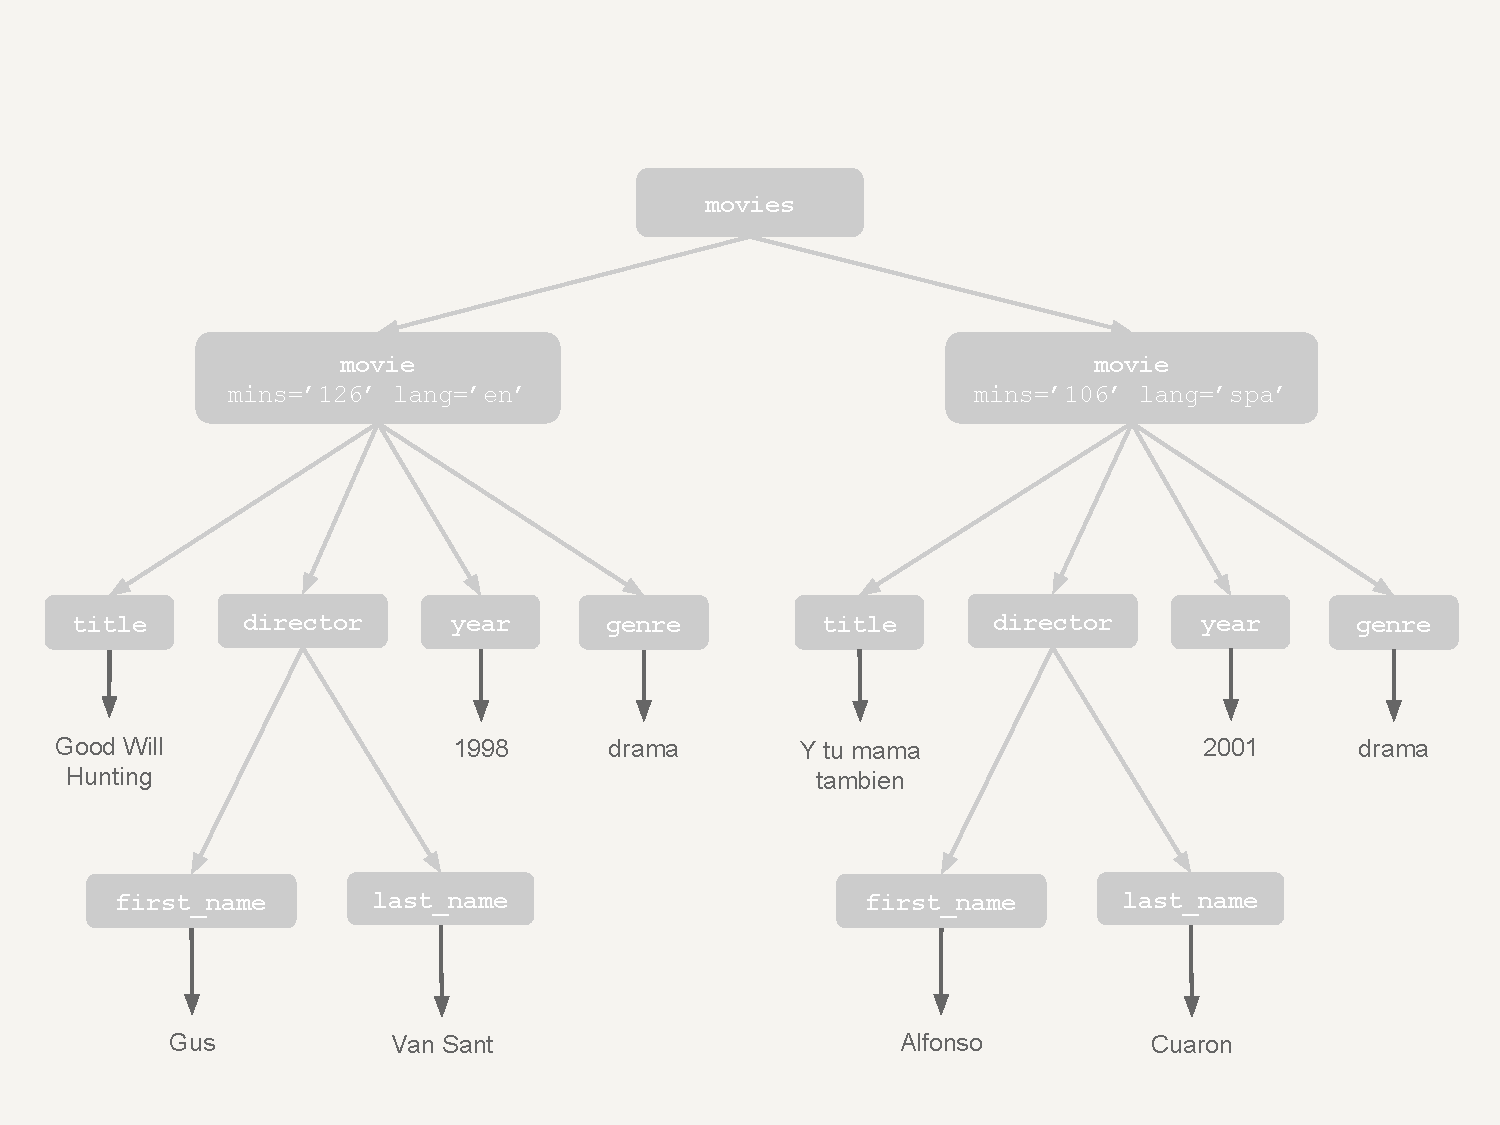
\includegraphics[width=10cm]{images/xpath_tree.pdf}
\end{center}

\end{frame}

%------------------------------------------------

\begin{frame}[fragile]
\frametitle{XPath: movie nodes}

\begin{center}
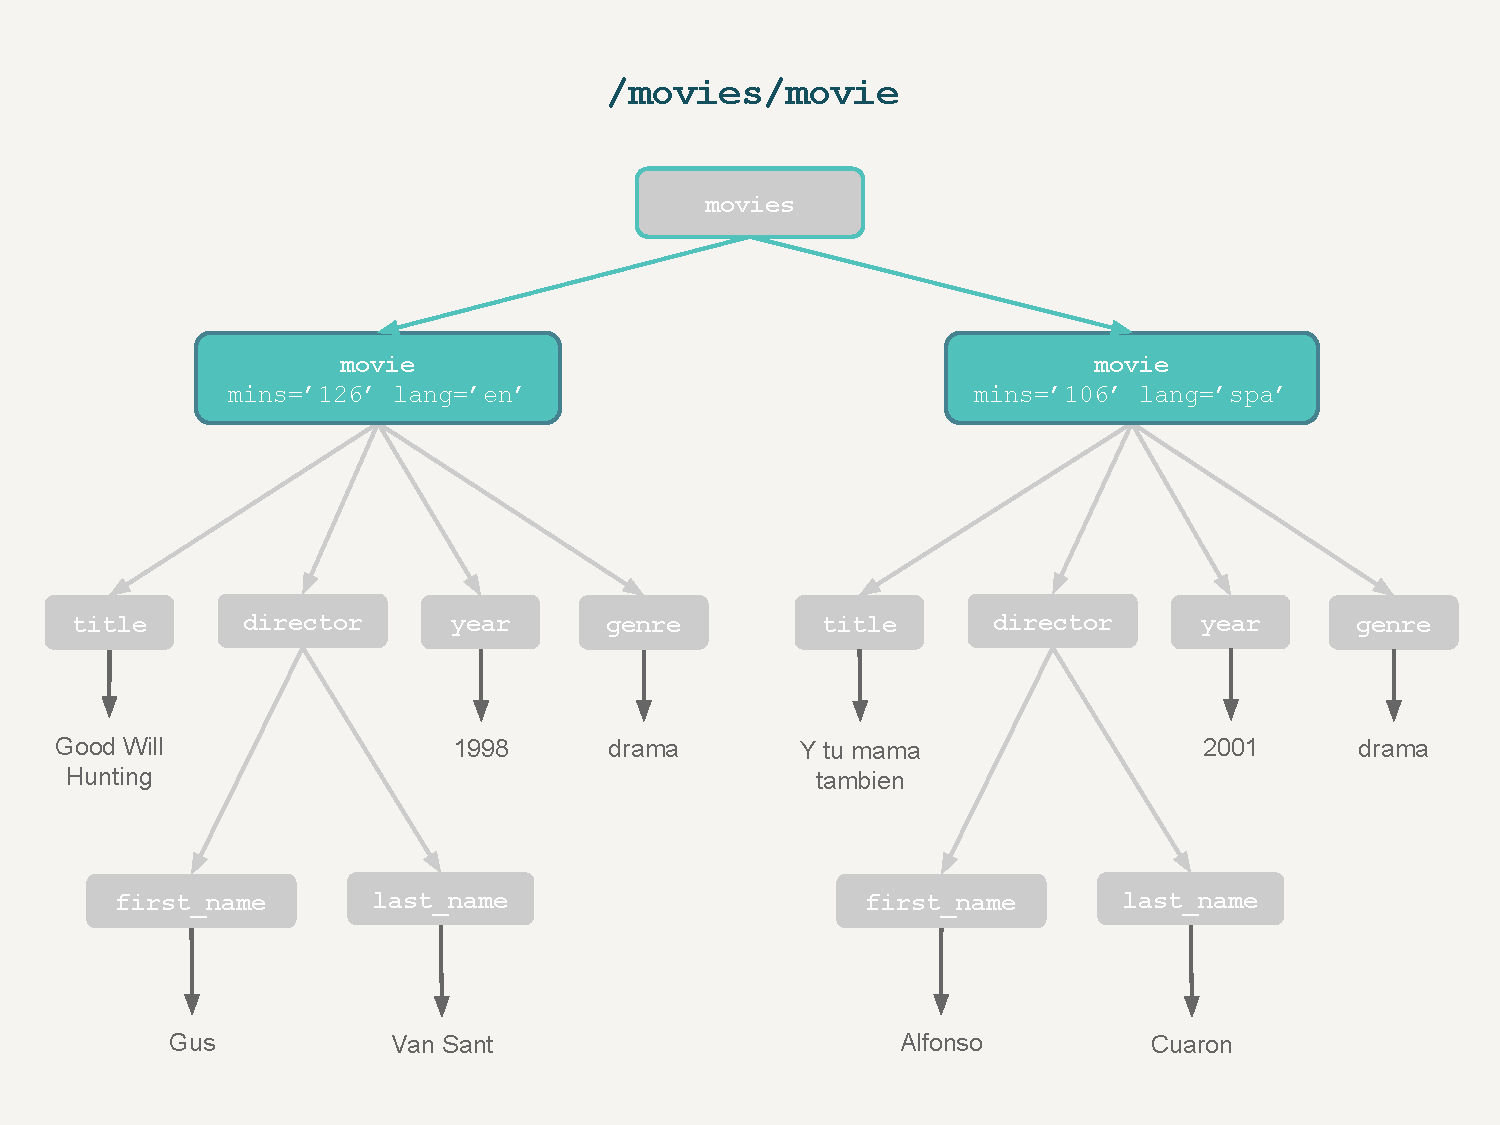
\includegraphics[width=10cm]{images/xpath_movie.pdf}
\end{center}

\end{frame}

%------------------------------------------------

\begin{frame}[fragile]
\frametitle{XPath: movie title nodes}

\begin{center}
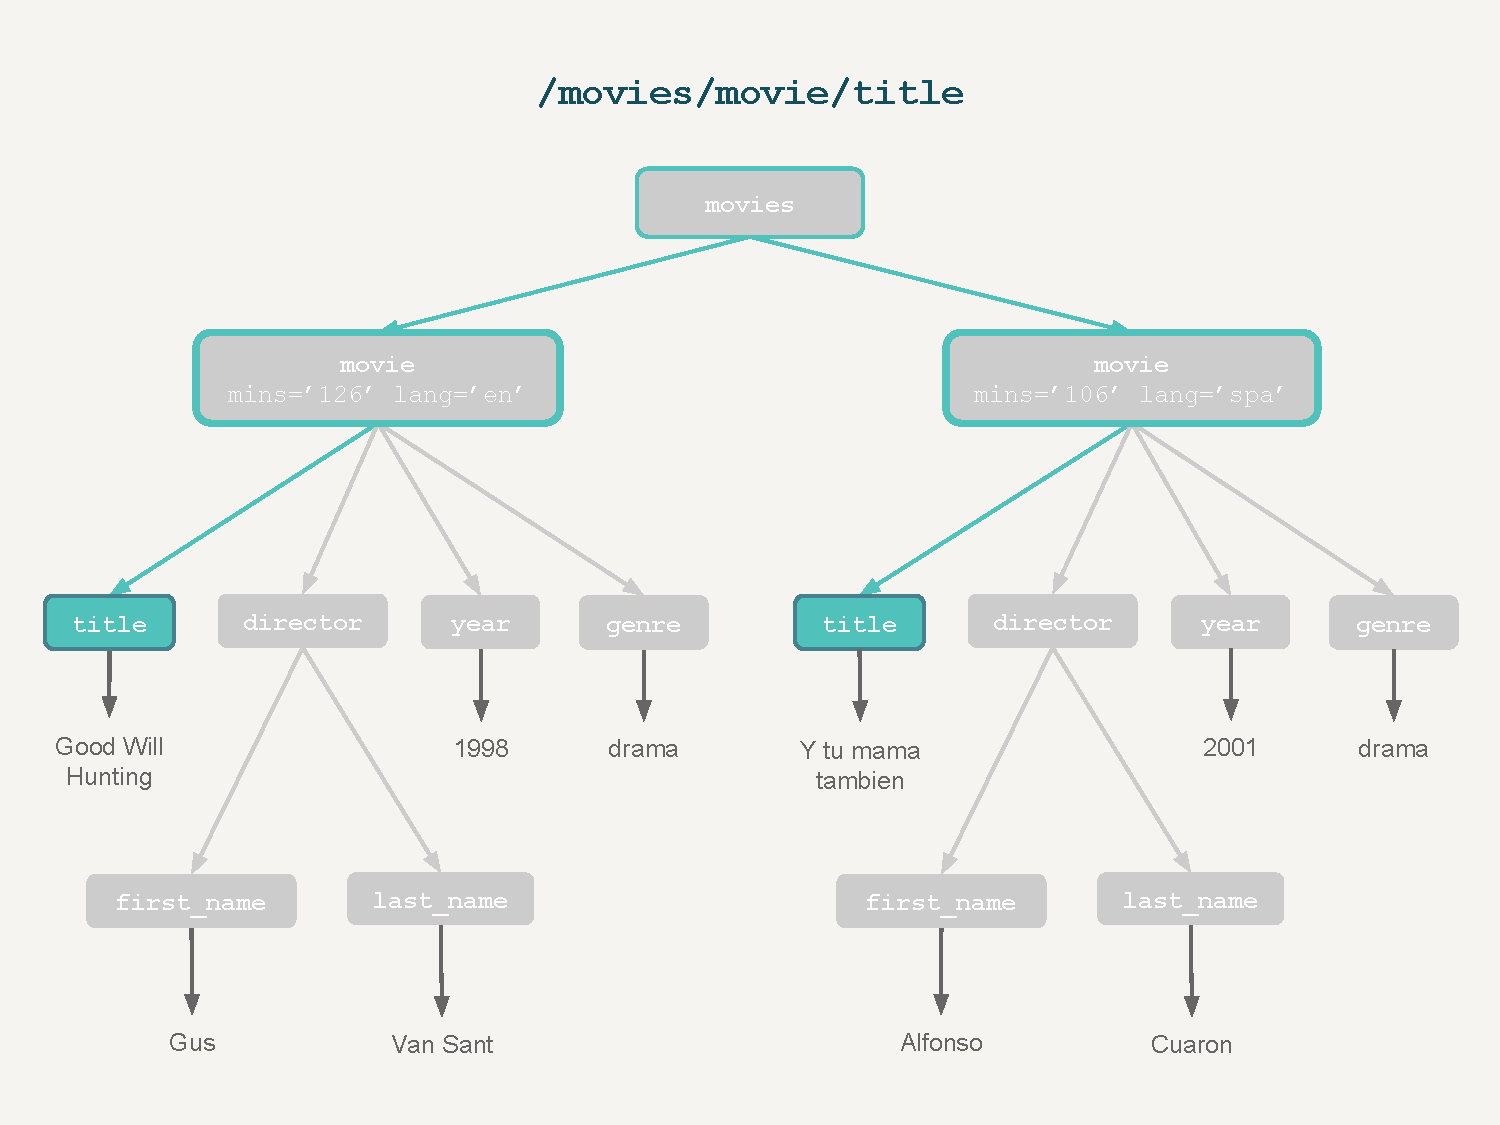
\includegraphics[width=10cm]{images/xpath_title.pdf}
\end{center}

\end{frame}

%------------------------------------------------

\begin{frame}[fragile]
\frametitle{XPath: movie director's first name nodes}

\begin{center}
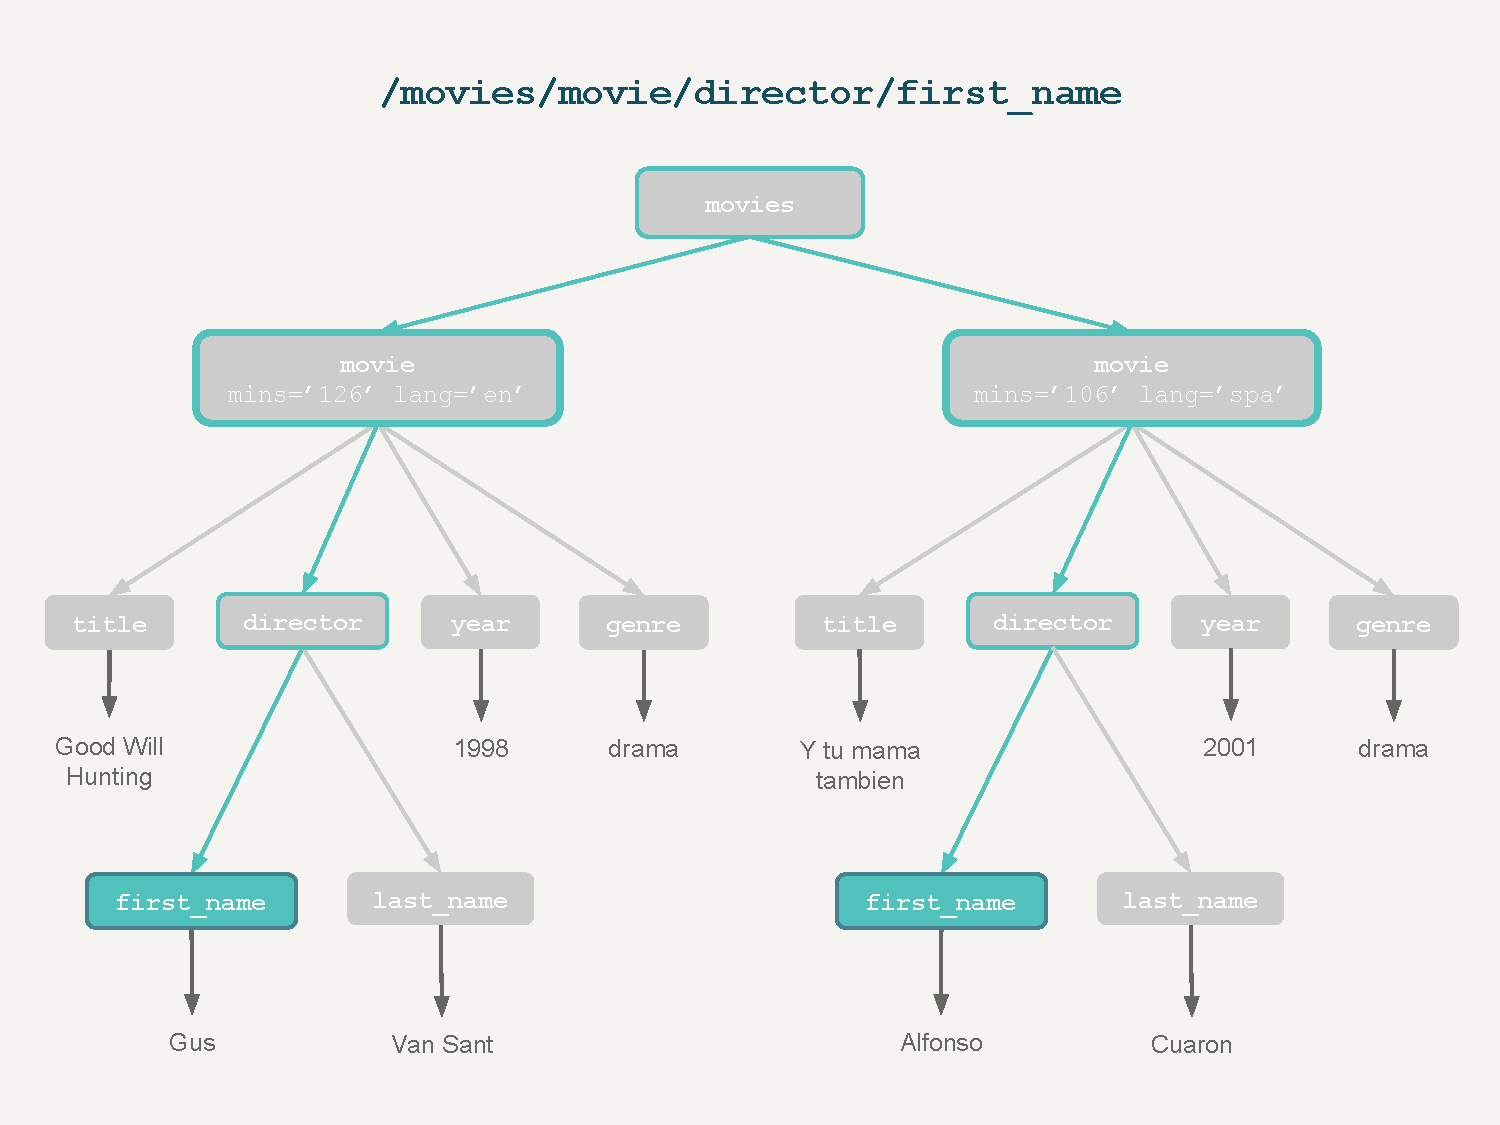
\includegraphics[width=10cm]{images/xpath_firstname.pdf}
\end{center}

\end{frame}

%------------------------------------------------

\begin{frame}[fragile]
\frametitle{XPath: movie director nodes}

\begin{center}
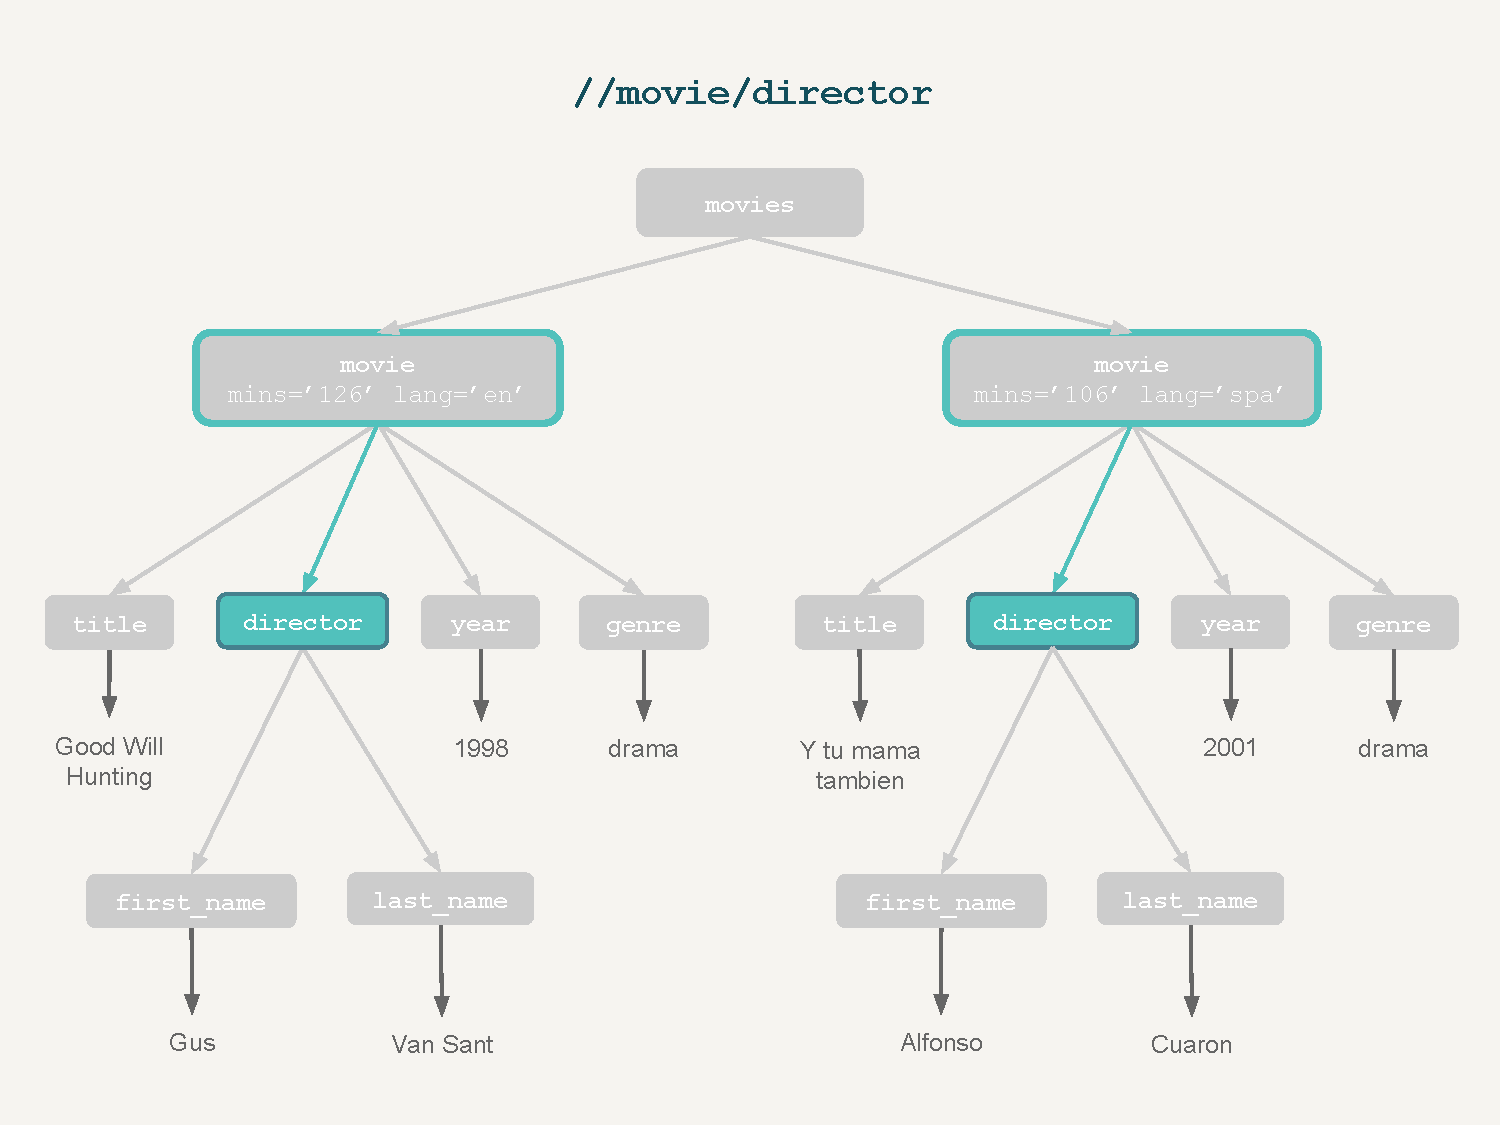
\includegraphics[width=10cm]{images/xpath_director.pdf}
\end{center}

\end{frame}

%------------------------------------------------

\begin{frame}[fragile]
\frametitle{XPath: last name nodes}

\begin{center}
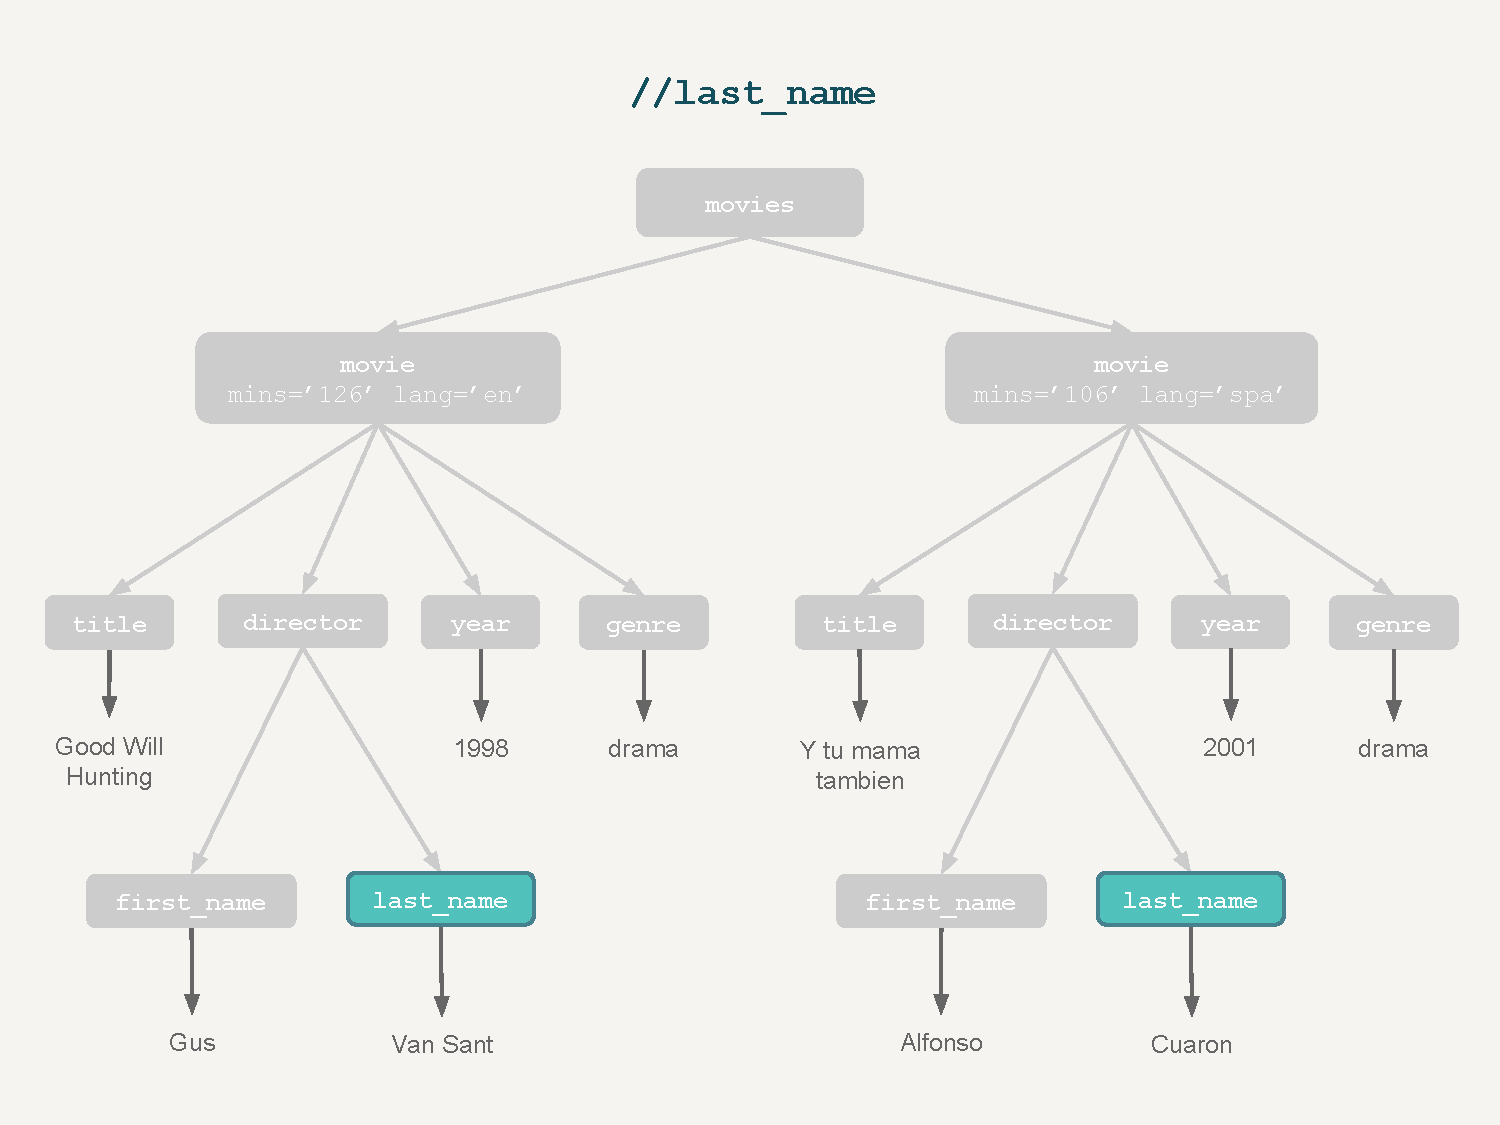
\includegraphics[width=10cm]{images/xpath_lastname.pdf}
\end{center}

\end{frame}

%------------------------------------------------

\begin{frame}[fragile]
\frametitle{XPath: itle node of movie in Spanish}

\begin{center}
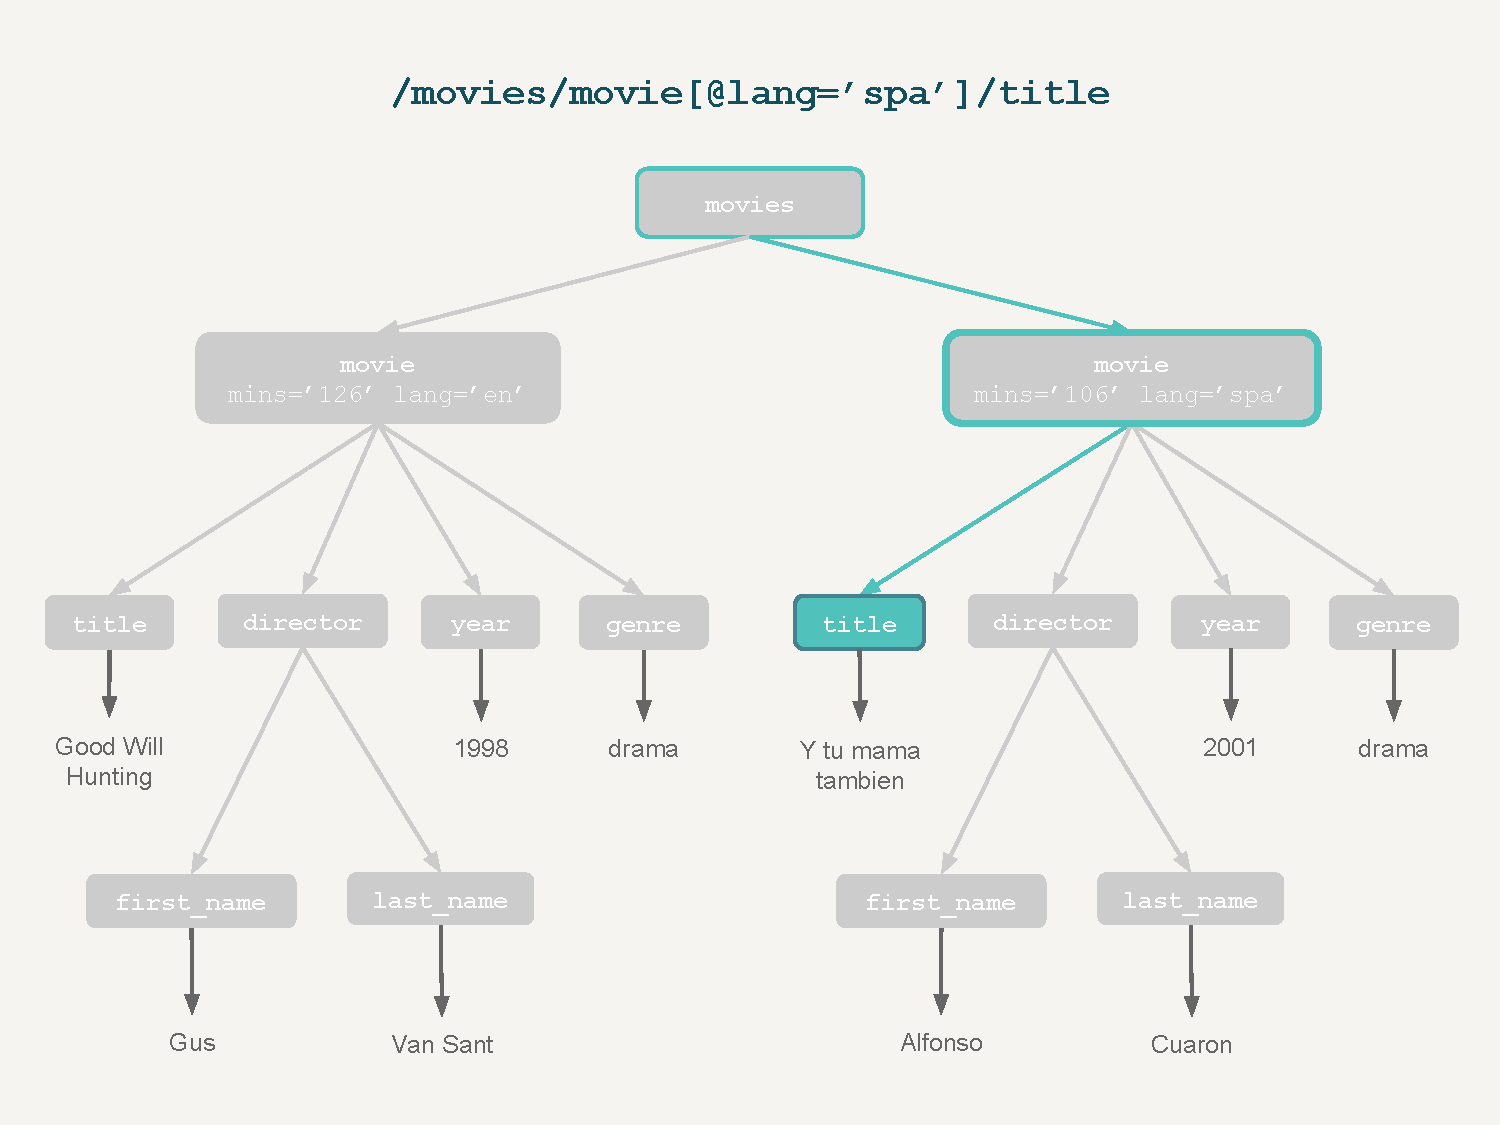
\includegraphics[width=10cm]{images/xpath_ytmt.pdf}
\end{center}

\end{frame}

%------------------------------------------------

\begin{frame}
 \begin{center}
  {\Huge \textcolor{mandarina}{Querying Parsed Documents}}
 \end{center}
\end{frame}

%------------------------------------------------

\begin{frame}[fragile]
\frametitle{XPath in "XML"}

\begin{block}{XPath in \code{"XML"}}
To work with XPath expressions using the \code{"XML"} package, we have the auxiliary function \highcode{getNodeSet()} that accepts XPath expressions in order to 
select node-sets. Its main usage is:
\begin{verbatim}
    getNodeSet(doc, path)
\end{verbatim}
\end{block}

where \highcode{doc} is an object of class \code{"XMLInternalDocument"} and \highcode{path} is a string giving the XPath expression to be evaluated

\end{frame}

%------------------------------------------------

\begin{frame}[fragile]
\frametitle{XML Movies Example}

\begin{columns}[t]
\begin{column}{0.5\textwidth}
\begin{knitrout}\tiny
\definecolor{shadecolor}{rgb}{1, 1, 1}\color{fgcolor}\begin{kframe}
\begin{alltt}
\hlcom{# define some xml content}
\hlstd{xml_string} \hlkwb{=} \hlkwd{c}\hlstd{(}
  \hlstr{'<?xml version="1.0" encoding="UTF-8"?>'}\hlstd{,}
  \hlstr{'<movies>'}\hlstd{,}
  \hlstr{'<movie mins="126" lang="eng">'}\hlstd{,}
  \hlstr{'<title>Good Will Hunting</title>'}\hlstd{,}
  \hlstr{'<director>'}\hlstd{,}
  \hlstr{'<first_name>Gus</first_name>'}\hlstd{,}
  \hlstr{'<last_name>Van Sant</last_name>'}\hlstd{,}
  \hlstr{'</director>'}\hlstd{,}
  \hlstr{'<year>1998</year>'}\hlstd{,}
  \hlstr{'<genre>drama</genre>'}\hlstd{,}
  \hlstr{'</movie>'}\hlstd{,}
  \hlstr{'<movie mins="106" lang="spa">'}\hlstd{,}
  \hlstr{'<title>Y tu mama tambien</title>'}\hlstd{,}
  \hlstr{'<director>'}\hlstd{,}
  \hlstr{'<first_name>Alfonso</first_name>'}\hlstd{,}
  \hlstr{'<last_name>Cuaron</last_name>'}\hlstd{,}
  \hlstr{'</director>'}\hlstd{,}
  \hlstr{'<year>2001</year>'}\hlstd{,}
  \hlstr{'<genre>drama</genre>'}\hlstd{,}
  \hlstr{'</movie>'}\hlstd{,}
  \hlstr{'</movies>'}\hlstd{)}

\hlcom{# parse xml content}
\hlstd{movies_xml} \hlkwb{=} \hlkwd{xmlParse}\hlstd{(xml_string,} \hlkwc{asText} \hlstd{=} \hlnum{TRUE}\hlstd{)}
\end{alltt}
\end{kframe}
\end{knitrout}
\end{column}

\begin{column}{0.5\textwidth}
\begin{knitrout}\tiny
\definecolor{shadecolor}{rgb}{1, 1, 1}\color{fgcolor}\begin{kframe}
\begin{alltt}
\hlcom{# check movies_xml}
\hlstd{movies_xml}
\end{alltt}
\begin{verbatim}
## <?xml version="1.0" encoding="UTF-8"?>
## <movies>
##   <movie mins="126" lang="eng">
##     <title>Good Will Hunting</title>
##     <director>
##       <first_name>Gus</first_name>
##       <last_name>Van Sant</last_name>
##     </director>
##     <year>1998</year>
##     <genre>drama</genre>
##   </movie>
##   <movie mins="106" lang="spa">
##     <title>Y tu mama tambien</title>
##     <director>
##       <first_name>Alfonso</first_name>
##       <last_name>Cuaron</last_name>
##     </director>
##     <year>2001</year>
##     <genre>drama</genre>
##   </movie>
## </movies>
## 
\end{verbatim}
\end{kframe}
\end{knitrout}
\end{column}
\end{columns}

\end{frame}

%------------------------------------------------

\begin{frame}[fragile]
\frametitle{Getting Nodes}

\begin{columns}[t]
\begin{column}{0.5\textwidth}
\begin{knitrout}\tiny
\definecolor{shadecolor}{rgb}{1, 1, 1}\color{fgcolor}\begin{kframe}
\begin{alltt}
\hlcom{# set of movie nodes}
\hlkwd{getNodeSet}\hlstd{(movies_xml,} \hlstr{"/movies/movie"}\hlstd{)}
\end{alltt}
\begin{verbatim}
## [[1]]
## <movie mins="126" lang="eng">
##   <title>Good Will Hunting</title>
##   <director>
##     <first_name>Gus</first_name>
##     <last_name>Van Sant</last_name>
##   </director>
##   <year>1998</year>
##   <genre>drama</genre>
## </movie> 
## 
## [[2]]
## <movie mins="106" lang="spa">
##   <title>Y tu mama tambien</title>
##   <director>
##     <first_name>Alfonso</first_name>
##     <last_name>Cuaron</last_name>
##   </director>
##   <year>2001</year>
##   <genre>drama</genre>
## </movie> 
## 
## attr(,"class")
## [1] "XMLNodeSet"
\end{verbatim}
\end{kframe}
\end{knitrout}
\end{column}

\begin{column}{0.5\textwidth}
\begin{knitrout}\tiny
\definecolor{shadecolor}{rgb}{1, 1, 1}\color{fgcolor}\begin{kframe}
\begin{alltt}
\hlcom{# equivalently}
\hlkwd{getNodeSet}\hlstd{(movies_xml,} \hlstr{"//movie"}\hlstd{)}
\end{alltt}
\begin{verbatim}
## [[1]]
## <movie mins="126" lang="eng">
##   <title>Good Will Hunting</title>
##   <director>
##     <first_name>Gus</first_name>
##     <last_name>Van Sant</last_name>
##   </director>
##   <year>1998</year>
##   <genre>drama</genre>
## </movie> 
## 
## [[2]]
## <movie mins="106" lang="spa">
##   <title>Y tu mama tambien</title>
##   <director>
##     <first_name>Alfonso</first_name>
##     <last_name>Cuaron</last_name>
##   </director>
##   <year>2001</year>
##   <genre>drama</genre>
## </movie> 
## 
## attr(,"class")
## [1] "XMLNodeSet"
\end{verbatim}
\end{kframe}
\end{knitrout}
\end{column}
\end{columns}

\end{frame}

%------------------------------------------------

\begin{frame}[fragile]
\frametitle{Getting Nodes}

\begin{columns}[t]
\begin{column}{0.5\textwidth}
\begin{knitrout}\tiny
\definecolor{shadecolor}{rgb}{1, 1, 1}\color{fgcolor}\begin{kframe}
\begin{alltt}
\hlcom{# set of title nodes}
\hlkwd{getNodeSet}\hlstd{(movies_xml,} \hlstr{"//title"}\hlstd{)}
\end{alltt}
\begin{verbatim}
## [[1]]
## <title>Good Will Hunting</title> 
## 
## [[2]]
## <title>Y tu mama tambien</title> 
## 
## attr(,"class")
## [1] "XMLNodeSet"
\end{verbatim}
\begin{alltt}
\hlcom{# set of year nodes}
\hlkwd{getNodeSet}\hlstd{(movies_xml,} \hlstr{"//year"}\hlstd{)}
\end{alltt}
\begin{verbatim}
## [[1]]
## <year>1998</year> 
## 
## [[2]]
## <year>2001</year> 
## 
## attr(,"class")
## [1] "XMLNodeSet"
\end{verbatim}
\end{kframe}
\end{knitrout}
\end{column}

\begin{column}{0.5\textwidth}
\begin{knitrout}\tiny
\definecolor{shadecolor}{rgb}{1, 1, 1}\color{fgcolor}\begin{kframe}
\begin{alltt}
\hlcom{# set of director nodes}
\hlkwd{getNodeSet}\hlstd{(movies_xml,} \hlstr{"//director"}\hlstd{)}
\end{alltt}
\begin{verbatim}
## [[1]]
## <director>
##   <first_name>Gus</first_name>
##   <last_name>Van Sant</last_name>
## </director> 
## 
## [[2]]
## <director>
##   <first_name>Alfonso</first_name>
##   <last_name>Cuaron</last_name>
## </director> 
## 
## attr(,"class")
## [1] "XMLNodeSet"
\end{verbatim}
\end{kframe}
\end{knitrout}
\end{column}
\end{columns}

\end{frame}

%------------------------------------------------

\begin{frame}[fragile]
\frametitle{Getting Nodes}

\begin{columns}[t]
\begin{column}{0.5\textwidth}
\begin{knitrout}\tiny
\definecolor{shadecolor}{rgb}{1, 1, 1}\color{fgcolor}\begin{kframe}
\begin{alltt}
\hlcom{# set of movie nodes with attribute lang = 'eng'}
\hlkwd{getNodeSet}\hlstd{(movies_xml,} \hlstr{"//movie[@lang='eng']"}\hlstd{)}
\end{alltt}
\begin{verbatim}
## [[1]]
## <movie mins="126" lang="eng">
##   <title>Good Will Hunting</title>
##   <director>
##     <first_name>Gus</first_name>
##     <last_name>Van Sant</last_name>
##   </director>
##   <year>1998</year>
##   <genre>drama</genre>
## </movie> 
## 
## attr(,"class")
## [1] "XMLNodeSet"
\end{verbatim}
\end{kframe}
\end{knitrout}
\end{column}

\begin{column}{0.5\textwidth}
\begin{knitrout}\tiny
\definecolor{shadecolor}{rgb}{1, 1, 1}\color{fgcolor}\begin{kframe}
\begin{alltt}
\hlcom{# set of movie nodes with attribute lang = 'spa'}
\hlkwd{getNodeSet}\hlstd{(movies_xml,} \hlstr{"//movie[@lang='spa']"}\hlstd{)}
\end{alltt}
\begin{verbatim}
## [[1]]
## <movie mins="106" lang="spa">
##   <title>Y tu mama tambien</title>
##   <director>
##     <first_name>Alfonso</first_name>
##     <last_name>Cuaron</last_name>
##   </director>
##   <year>2001</year>
##   <genre>drama</genre>
## </movie> 
## 
## attr(,"class")
## [1] "XMLNodeSet"
\end{verbatim}
\end{kframe}
\end{knitrout}
\end{column}
\end{columns}

\end{frame}

%------------------------------------------------

\begin{frame}
 \begin{center}
  {\Huge \textcolor{mandarina}{Case Study}}
 \end{center}
\end{frame}

%------------------------------------------------

\begin{frame}
\frametitle{R Mailing Lists}

\begin{center}
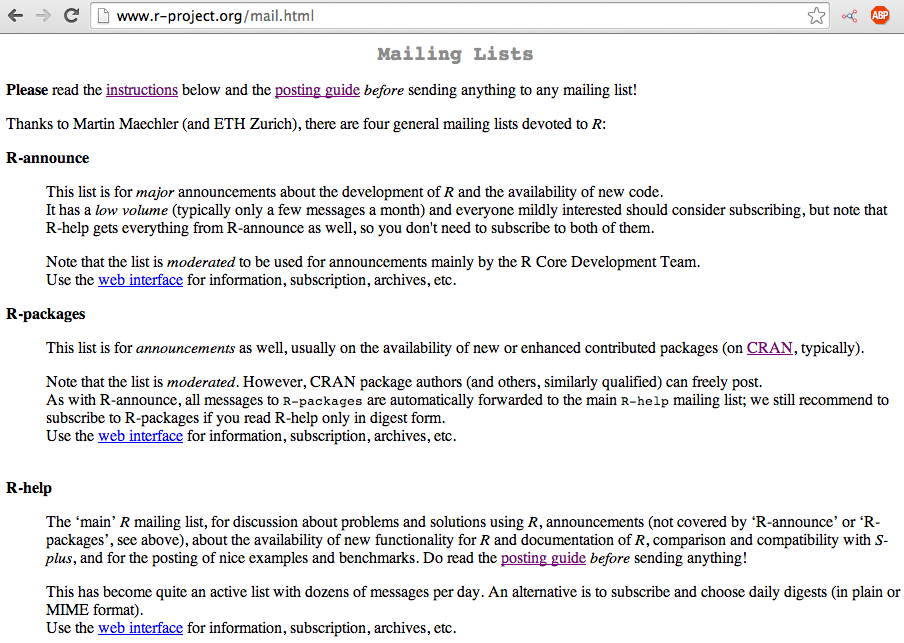
\includegraphics[width=10cm]{images/mailing_lists.png}
\end{center}

\end{frame}

%------------------------------------------------

\begin{frame}[fragile]
\frametitle{Parsing HTML document}

Let's parse the R mailing lists page: \\
{\scriptsize \url{http://www.r-project.org/mail.html}}

\begin{knitrout}\tiny
\definecolor{shadecolor}{rgb}{1, 1, 1}\color{fgcolor}\begin{kframe}
\begin{alltt}
\hlcom{# R mailing lists url}
\hlstd{mailing_url} \hlkwb{=} \hlstr{"http://www.r-project.org/mail.html"}

\hlcom{# parse html content}
\hlstd{mailing_doc} \hlkwb{=} \hlkwd{htmlParse}\hlstd{(mailing_url)}
\end{alltt}
\end{kframe}
\end{knitrout}



\begin{knitrout}\tiny
\definecolor{shadecolor}{rgb}{1, 1, 1}\color{fgcolor}\begin{kframe}
\begin{alltt}
\hlcom{# check class 'HTMLInternalDocument'}
\hlkwd{class}\hlstd{(mailing_doc)}
\end{alltt}
\begin{verbatim}
## [1] "HTMLInternalDocument" "HTMLInternalDocument" "XMLInternalDocument" 
## [4] "XMLAbstractDocument"
\end{verbatim}
\begin{alltt}
\hlcom{# get root node}
\hlstd{mailing_root} \hlkwb{=} \hlkwd{xmlRoot}\hlstd{(mailing_doc)}
\end{alltt}
\end{kframe}
\end{knitrout}

\end{frame}

%------------------------------------------------

\begin{frame}[fragile]
\frametitle{Inspecting Root Node}

Let's inspect the Root Node
\begin{knitrout}\tiny
\definecolor{shadecolor}{rgb}{1, 1, 1}\color{fgcolor}\begin{kframe}
\begin{alltt}
\hlcom{# how many child nodes in root}
\hlkwd{xmlSize}\hlstd{(mailing_root)}
\end{alltt}
\begin{verbatim}
## [1] 2
\end{verbatim}
\begin{alltt}
\hlcom{# names of root child nodes}
\hlkwd{xmlSApply}\hlstd{(mailing_root, xmlName)}
\end{alltt}
\begin{verbatim}
##   head   body 
## "head" "body"
\end{verbatim}
\begin{alltt}
\hlcom{# how many nodes in each children}
\hlkwd{xmlSApply}\hlstd{(mailing_root, xmlSize)}
\end{alltt}
\begin{verbatim}
## head body 
##    2   23
\end{verbatim}
\end{kframe}
\end{knitrout}

\end{frame}

%------------------------------------------------

\begin{frame}[fragile]
\frametitle{Getting HTML body element}

\begin{knitrout}\tiny
\definecolor{shadecolor}{rgb}{1, 1, 1}\color{fgcolor}\begin{kframe}
\begin{alltt}
\hlcom{# get the html body node}
\hlstd{mailing_body} \hlkwb{=} \hlkwd{xmlChildren}\hlstd{(mailing_root)}\hlopt{$}\hlstd{body}

\hlcom{# get all 'h1' elements}
\hlkwd{xpathSApply}\hlstd{(mailing_body,} \hlstr{"h1"}\hlstd{)}
\end{alltt}
\begin{verbatim}
## [[1]]
## <h1>Mailing Lists</h1>
\end{verbatim}
\begin{alltt}
\hlcom{# get all 'h2' elements}
\hlkwd{xpathSApply}\hlstd{(mailing_body,} \hlstr{"h2"}\hlstd{)}
\end{alltt}
\begin{verbatim}
## [[1]]
## <h2>Archives and Search Facilities</h2>
\end{verbatim}
\end{kframe}
\end{knitrout}

\end{frame}

%------------------------------------------------

\begin{frame}
\frametitle{Special Interest Group}

\begin{center}
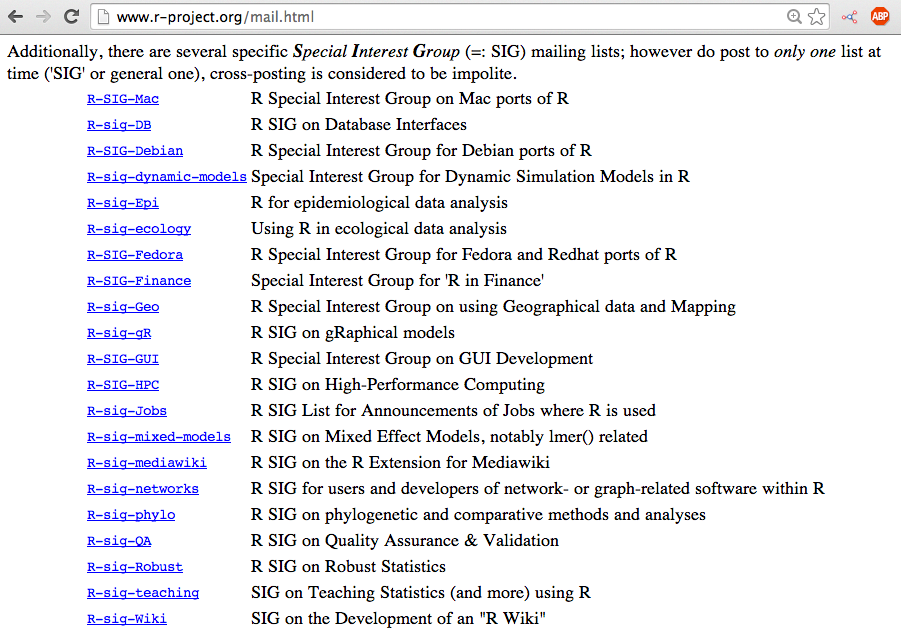
\includegraphics[width=10cm]{images/mailing_sig.png}
\end{center}

\end{frame}

%------------------------------------------------

\begin{frame}
\frametitle{Special Interest Group}

Take a look at the source code: note that it is a \highcode{table} node

\begin{center}
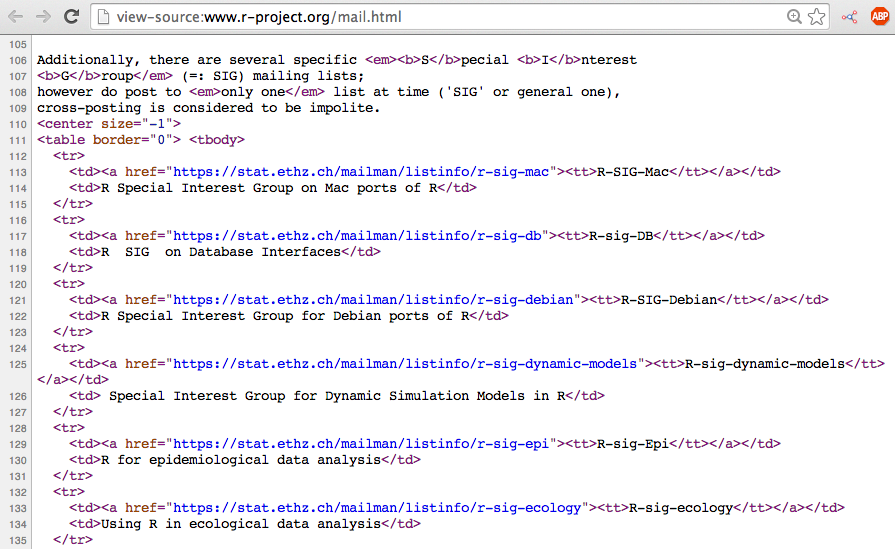
\includegraphics[width=9cm]{images/mailing_sig_source.png}
\end{center}

\end{frame}

%------------------------------------------------

\begin{frame}[fragile]
\frametitle{Getting "Special Interest Groups"}

Let's work with the \textit{Special Interest Groups} section. We can read the content of the table with \highcode{readHTMLTable()}

\begin{knitrout}\tiny
\definecolor{shadecolor}{rgb}{1, 1, 1}\color{fgcolor}\begin{kframe}
\begin{alltt}
\hlcom{# get the html table "Special Interest Groups"}
\hlstd{sig_content} \hlkwb{=} \hlkwd{readHTMLTable}\hlstd{(mailing_doc,} \hlkwc{which} \hlstd{=} \hlnum{1}\hlstd{)}

\hlkwd{head}\hlstd{(sig_content)}
\end{alltt}
\begin{verbatim}
##                     V1
## 1            R-SIG-Mac
## 2             R-sig-DB
## 3         R-SIG-Debian
## 4 R-sig-dynamic-models
## 5            R-sig-Epi
## 6        R-sig-ecology
##                                                          V2
## 1                R Special Interest Group on Mac ports of R
## 2                            R  SIG  on Database Interfaces
## 3            R Special Interest Group for Debian ports of R
## 4 Special Interest Group for Dynamic Simulation Models in R
## 5                       R for epidemiological data analysis
## 6                       Using R in ecological data analysis
\end{verbatim}
\end{kframe}
\end{knitrout}

\end{frame}

%------------------------------------------------

\begin{frame}[fragile]
\frametitle{Getting "Special Interest Groups" (SIG)}

We can also work with XPath expressions in order to get the information contained in the table of \textit{Special Interest Groups}

\bigskip

For instance, let's work with the \highcode{a} elements in the \highcode{table} \low{(i.e. the links)}

\begin{knitrout}\tiny
\definecolor{shadecolor}{rgb}{1, 1, 1}\color{fgcolor}\begin{kframe}
\begin{alltt}
\hlcom{# SIG table from doc 'HTMLInternalDocument'}
\hlstd{sig_from_doc} \hlkwb{=} \hlkwd{xpathSApply}\hlstd{(mailing_doc,} \hlstr{"//table/..//a"}\hlstd{)}

\hlcom{# SIG table from root 'XMLInternalElementNode'}
\hlstd{sig_from_root} \hlkwb{=} \hlkwd{xpathSApply}\hlstd{(mailing_root,} \hlstr{"//table/..//a"}\hlstd{)}
\end{alltt}
\end{kframe}
\end{knitrout}

\end{frame}

%------------------------------------------------

\begin{frame}[fragile]
\frametitle{Getting "Special Interest Groups" (SIG)}

Let's compare the results:
\begin{knitrout}\tiny
\definecolor{shadecolor}{rgb}{1, 1, 1}\color{fgcolor}\begin{kframe}
\begin{alltt}
\hlkwd{head}\hlstd{(sig_from_doc,} \hlkwc{n} \hlstd{=} \hlnum{2}\hlstd{)}
\end{alltt}
\begin{verbatim}
## [[1]]
## <a href="https://stat.ethz.ch/mailman/listinfo/r-sig-mac">
##   <tt>R-SIG-Mac</tt>
## </a> 
## 
## [[2]]
## <a href="https://stat.ethz.ch/mailman/listinfo/r-sig-db">
##   <tt>R-sig-DB</tt>
## </a>
\end{verbatim}
\begin{alltt}
\hlkwd{head}\hlstd{(sig_from_root,} \hlkwc{n} \hlstd{=} \hlnum{2}\hlstd{)}
\end{alltt}
\begin{verbatim}
## [[1]]
## <a href="https://stat.ethz.ch/mailman/listinfo/r-sig-mac">
##   <tt>R-SIG-Mac</tt>
## </a> 
## 
## [[2]]
## <a href="https://stat.ethz.ch/mailman/listinfo/r-sig-db">
##   <tt>R-sig-DB</tt>
## </a>
\end{verbatim}
\end{kframe}
\end{knitrout}

\end{frame}

%------------------------------------------------

\begin{frame}[fragile]
\frametitle{Getting "Special Interest Groups" (SIG)}

Here's one way to get the link names of the Special Interest Groups \low{(ie values in the first column of the html table)}
\begin{knitrout}\tiny
\definecolor{shadecolor}{rgb}{1, 1, 1}\color{fgcolor}\begin{kframe}
\begin{alltt}
\hlcom{# names of SIG links}
\hlkwd{sapply}\hlstd{(sig_from_root, xmlValue)}
\end{alltt}
\begin{verbatim}
##  [1] "R-SIG-Mac"            "R-sig-DB"             "R-SIG-Debian"        
##  [4] "R-sig-dynamic-models" "R-sig-Epi"            "R-sig-ecology"       
##  [7] "R-SIG-Fedora"         "R-SIG-Finance"        "R-sig-Geo"           
## [10] "R-sig-gR"             "R-SIG-GUI"            "R-SIG-HPC"           
## [13] "R-sig-Jobs"           "R-sig-mixed-models"   "R-sig-mediawiki"     
## [16] "R-sig-networks"       "R-sig-phylo"          "R-sig-QA"            
## [19] "R-sig-Robust"         "R-sig-teaching"       "R-sig-Wiki"
\end{verbatim}
\end{kframe}
\end{knitrout}

\end{frame}

%------------------------------------------------

\begin{frame}[fragile]
\frametitle{Getting "Special Interest Groups" (SIG)}

Extracting \highcode{a} elements in \highcode{table}
\begin{knitrout}\tiny
\definecolor{shadecolor}{rgb}{1, 1, 1}\color{fgcolor}\begin{kframe}
\begin{alltt}
\hlcom{# XPath expression to extract 'a' nodes}
\hlstd{sig_links} \hlkwb{=} \hlkwd{xpathSApply}\hlstd{(mailing_root,} \hlstr{"//table/..//a"}\hlstd{)}
\hlkwd{head}\hlstd{(sig_links,} \hlkwc{n} \hlstd{=} \hlnum{4}\hlstd{)}
\end{alltt}
\begin{verbatim}
## [[1]]
## <a href="https://stat.ethz.ch/mailman/listinfo/r-sig-mac">
##   <tt>R-SIG-Mac</tt>
## </a> 
## 
## [[2]]
## <a href="https://stat.ethz.ch/mailman/listinfo/r-sig-db">
##   <tt>R-sig-DB</tt>
## </a> 
## 
## [[3]]
## <a href="https://stat.ethz.ch/mailman/listinfo/r-sig-debian">
##   <tt>R-SIG-Debian</tt>
## </a> 
## 
## [[4]]
## <a href="https://stat.ethz.ch/mailman/listinfo/r-sig-dynamic-models">
##   <tt>R-sig-dynamic-models</tt>
## </a>
\end{verbatim}
\end{kframe}
\end{knitrout}

\end{frame}

%------------------------------------------------

\begin{frame}[fragile]
\frametitle{Getting "Special Interest Groups" (SIG)}

Extracting attributes from \highcode{a} elements in \highcode{table}
\begin{knitrout}\tiny
\definecolor{shadecolor}{rgb}{1, 1, 1}\color{fgcolor}\begin{kframe}
\begin{alltt}
\hlcom{# XPath expression attributes of nodes}
\hlstd{sig_link_attrs} \hlkwb{=} \hlkwd{xpathSApply}\hlstd{(mailing_root,} \hlstr{"//table/..//a"}\hlstd{, xmlAttrs)}
\hlkwd{head}\hlstd{(sig_link_attrs)}
\end{alltt}
\begin{verbatim}
##                                                         href 
##            "https://stat.ethz.ch/mailman/listinfo/r-sig-mac" 
##                                                         href 
##             "https://stat.ethz.ch/mailman/listinfo/r-sig-db" 
##                                                         href 
##         "https://stat.ethz.ch/mailman/listinfo/r-sig-debian" 
##                                                         href 
## "https://stat.ethz.ch/mailman/listinfo/r-sig-dynamic-models" 
##                                                         href 
##            "https://stat.ethz.ch/mailman/listinfo/r-sig-epi" 
##                                                         href 
##        "https://stat.ethz.ch/mailman/listinfo/r-sig-ecology"
\end{verbatim}
\end{kframe}
\end{knitrout}

\end{frame}

%------------------------------------------------

\begin{frame}[fragile]
\frametitle{Getting "Special Interest Groups" (SIG)}

Extracting values from \highcode{href} attributes of \highcode{a} elements in \highcode{table}
\begin{knitrout}\tiny
\definecolor{shadecolor}{rgb}{1, 1, 1}\color{fgcolor}\begin{kframe}
\begin{alltt}
\hlcom{# XPath expression to extract attribute values of nodes}
\hlstd{sig_link_attr_vals} \hlkwb{=} \hlkwd{xpathSApply}\hlstd{(mailing_root,} \hlstr{"//table/..//a"}\hlstd{,}
                                 \hlstd{xmlGetAttr,} \hlstr{"href"}\hlstd{)}
\hlkwd{head}\hlstd{(sig_link_attr_vals,} \hlkwc{n} \hlstd{=} \hlnum{10}\hlstd{)}
\end{alltt}
\begin{verbatim}
##  [1] "https://stat.ethz.ch/mailman/listinfo/r-sig-mac"           
##  [2] "https://stat.ethz.ch/mailman/listinfo/r-sig-db"            
##  [3] "https://stat.ethz.ch/mailman/listinfo/r-sig-debian"        
##  [4] "https://stat.ethz.ch/mailman/listinfo/r-sig-dynamic-models"
##  [5] "https://stat.ethz.ch/mailman/listinfo/r-sig-epi"           
##  [6] "https://stat.ethz.ch/mailman/listinfo/r-sig-ecology"       
##  [7] "https://stat.ethz.ch/mailman/listinfo/r-sig-fedora"        
##  [8] "https://stat.ethz.ch/mailman/listinfo/r-sig-finance"       
##  [9] "https://stat.ethz.ch/mailman/listinfo/r-sig-geo"           
## [10] "https://stat.ethz.ch/mailman/listinfo/r-sig-gr"
\end{verbatim}
\end{kframe}
\end{knitrout}

\end{frame}

%------------------------------------------------

\begin{frame}[fragile]
\frametitle{Getting "Special Interest Groups" (SIG)}

Extracting content from \highcode{a} elements in \highcode{table}
\begin{knitrout}\tiny
\definecolor{shadecolor}{rgb}{1, 1, 1}\color{fgcolor}\begin{kframe}
\begin{alltt}
\hlcom{# XPath expression to extract content from nodes}
\hlstd{sig_link_values} \hlkwb{=} \hlkwd{xpathSApply}\hlstd{(mailing_root,} \hlstr{"//table/..//a"}\hlstd{, xmlValue)}

\hlstd{sig_link_values}
\end{alltt}
\begin{verbatim}
##  [1] "R-SIG-Mac"            "R-sig-DB"             "R-SIG-Debian"        
##  [4] "R-sig-dynamic-models" "R-sig-Epi"            "R-sig-ecology"       
##  [7] "R-SIG-Fedora"         "R-SIG-Finance"        "R-sig-Geo"           
## [10] "R-sig-gR"             "R-SIG-GUI"            "R-SIG-HPC"           
## [13] "R-sig-Jobs"           "R-sig-mixed-models"   "R-sig-mediawiki"     
## [16] "R-sig-networks"       "R-sig-phylo"          "R-sig-QA"            
## [19] "R-sig-Robust"         "R-sig-teaching"       "R-sig-Wiki"
\end{verbatim}
\end{kframe}
\end{knitrout}

\end{frame}

%------------------------------------------------

\begin{frame}[fragile]
\frametitle{Getting "Special Interest Groups" (SIG)}

Extracting second \highcode{td} elements in \highcode{table} \low{(ie those containing the desccription of the SIGs)}
\begin{knitrout}\tiny
\definecolor{shadecolor}{rgb}{1, 1, 1}\color{fgcolor}\begin{kframe}
\begin{alltt}
\hlcom{# XPath expression to extract SIG descriptions}
\hlstd{sig_desc_nodes} \hlkwb{=} \hlkwd{xpathSApply}\hlstd{(mailing_root,} \hlstr{"//table/tbody/tr/td[2]"}\hlstd{)}

\hlkwd{head}\hlstd{(sig_desc_nodes,} \hlkwc{n} \hlstd{=} \hlnum{5}\hlstd{)}
\end{alltt}
\begin{verbatim}
## [[1]]
## <td>R Special Interest Group on Mac ports of R</td> 
## 
## [[2]]
## <td>R  SIG  on Database Interfaces</td> 
## 
## [[3]]
## <td>R Special Interest Group for Debian ports of R</td> 
## 
## [[4]]
## <td> Special Interest Group for Dynamic Simulation Models in R</td> 
## 
## [[5]]
## <td>R for epidemiological data analysis</td>
\end{verbatim}
\end{kframe}
\end{knitrout}

\end{frame}
%------------------------------------------------

\begin{frame}[fragile]
\frametitle{Getting "Special Interest Groups" (SIG)}

Extracting the content from the second \highcode{td} elements in \highcode{table} \low{(ie the actual desccription of the SIGs)}
\begin{knitrout}\tiny
\definecolor{shadecolor}{rgb}{1, 1, 1}\color{fgcolor}\begin{kframe}
\begin{alltt}
\hlcom{# XPath expression to extract SIG descriptions}
\hlstd{sig_descriptions} \hlkwb{=} \hlkwd{xpathSApply}\hlstd{(mailing_root,} \hlstr{"//table/tbody/tr/td[2]"}\hlstd{,}
                               \hlstd{xmlValue)}

\hlkwd{head}\hlstd{(sig_descriptions,} \hlkwc{n} \hlstd{=} \hlnum{10}\hlstd{)}
\end{alltt}
\begin{verbatim}
##  [1] "R Special Interest Group on Mac ports of R"                     
##  [2] "R  SIG  on Database Interfaces"                                 
##  [3] "R Special Interest Group for Debian ports of R"                 
##  [4] " Special Interest Group for Dynamic Simulation Models in R"     
##  [5] "R for epidemiological data analysis"                            
##  [6] "Using R in ecological data analysis"                            
##  [7] "R Special Interest Group for Fedora and Redhat ports of R"      
##  [8] "Special Interest Group for 'R in Finance'"                      
##  [9] "R Special Interest Group on using Geographical data and Mapping"
## [10] "R  SIG  on  gRaphical models"
\end{verbatim}
\end{kframe}
\end{knitrout}

\end{frame}

%------------------------------------------------

\end{document}
